\documentclass{article}
%%%%%%%%%%%%%%%%%%%%%%%%%%%%%%%%%%%%%%%%%%%%%%%%%%%%%%%%%%%%%%%%%%%%%%%%%%%%%%%%%%%%%%%%%%%%%%%%%%%%%%%%%
\usepackage{csquotes,xpatch}% recommended
\usepackage[backend=bibtex,
style=authoryear-comp,
sortcites=false,
maxbibnames=5,maxcitenames=2,
firstinits=true,
natbib=true,
]{biblatex}

\addbibresource{refs.bib}

% natbib = true: add comma between author and year
% firstinits: for first name initials in bibliography
\renewcommand{\postnotedelim}{ } % remove comma in post citation in autocite
%\addbibresource{refs.bib}
%%%%%%%%%%%%%%%%%%%%%%%%%%%%%%%%%%%%%%%%%%%%%%%%%%%%%%%%%%%%%%%%%%%%%%%%%%%%%%%%%%%%%%%%%%%%%%%%%%%%%%%%%

% Combine label and labelyear links
\xpatchbibmacro{cite}
{\usebibmacro{cite:label}%
	\setunit{\addspace}%
	\usebibmacro{cite:labelyear+extrayear}}
{\printtext[bibhyperref]{%
		\DeclareFieldAlias{bibhyperref}{default}%
		\usebibmacro{cite:label}%
		\setunit{\addspace}%
		\usebibmacro{cite:labelyear+extrayear}}}{}{}

% Include labelname in labelyear link
\xpatchbibmacro{cite}
{\printnames{labelname}%
	\setunit{\nameyeardelim}%
	\usebibmacro{cite:labelyear+extrayear}}
{\printtext[bibhyperref]{%
		\DeclareFieldAlias{bibhyperref}{default}%
		\printnames{labelname}%
		\setunit{\nameyeardelim}%
		\usebibmacro{cite:labelyear+extrayear}}}{}{}

% Access hyperref's citation link start/end commands
\makeatletter
\protected\def\blx@imc@biblinkstart{%
	\@ifnextchar[%]
	{\blx@biblinkstart}
	{\blx@biblinkstart[\abx@field@entrykey]}}
\def\blx@biblinkstart[#1]{%
	\blx@sfsave\hyper@natlinkstart{\the\c@refsection @#1}\blx@sfrest}
\protected\def\blx@imc@biblinkend{%
	\blx@sfsave\hyper@natlinkend\blx@sfrest}
\blx@regimcs{\biblinkstart \biblinkend}
\makeatother

\newbool{cbx:link}

% Include parentheses around labelyear in \textcite only in
% single citations without pre- and postnotes
\def\iflinkparens{%
	\ifboolexpr{ test {\ifnumequal{\value{multicitetotal}}{0}} and
		test {\ifnumequal{\value{citetotal}}{1}} and
		test {\iffieldundef{prenote}} and
		test {\iffieldundef{postnote}} }}

\xpatchbibmacro{textcite}
{\printnames{labelname}}
{\iflinkparens
	{\DeclareFieldAlias{bibhyperref}{default}%
		\global\booltrue{cbx:link}\biblinkstart%
		\printnames{labelname}}
	{\printtext[bibhyperref]{\printnames{labelname}}}}{}{}

\xpatchbibmacro{textcite}
{\usebibmacro{cite:label}}
{\iflinkparens
	{\DeclareFieldAlias{bibhyperref}{default}%
		\global\booltrue{cbx:link}\biblinkstart%
		\usebibmacro{cite:label}}
	{\usebibmacro{cite:label}}}{}{}

\xpretobibmacro{textcite:postnote}
{\ifbool{cbx:link}% patch 2.7+
	{\ifbool{cbx:parens}
		{\bibcloseparen\global\boolfalse{cbx:parens}}
		{}%
		\biblinkend\global\boolfalse{cbx:link}}
	{}}
{}
{\xpatchbibmacro{textcite}% patch earlier releases
	{\setunit{%
			\ifbool{cbx:parens}
			{\bibcloseparen\global\boolfalse{cbx:parens}}
			{}%
			\multicitedelim}}
	{\ifbool{cbx:link}
		{\ifbool{cbx:parens}
			{\bibcloseparen\global\boolfalse{cbx:parens}}
			{}%
			\biblinkend\global\boolfalse{cbx:link}}
		{}%
		\setunit{%
			\ifbool{cbx:parens}
			{\bibcloseparen\global\boolfalse{cbx:parens}}
			{}%
			\multicitedelim}}
	{}{}}
%%%%%%%%%%%%%%%%%%%%%%%%%%%%%%%%%%%%%%%%%%%%%%%%%%%%%%%%%%%%%%%%%%%%%%%%%%%%%%%%%%%%%%%%%%%%%%%%%%%%%%%%%
\DeclareNameAlias{sortname}{last-first} % last name first
\renewbibmacro{in:}{} % remove in: before journal

%%%%%%%%%%%%%%%%%%%%%%%%%%%%%%%%%%%%%%%%%%%%%%%%%%%%%%%%%%%%%%%%%%%%%%%%%%%%%%%%%%%%%%%%%%%%%%%%%%%%%%%%%
\usepackage{graphicx}
\usepackage{epstopdf} 
%%%%%%%%%%%%%%%%%%%%%%%%%%%%%%%%%%%%%%%%%%%%%%%%%%%%%%%%%%%%%%%%%%%%%%%%%%%%%%%%%%%%%%%%%%%%%%%%%%%%%%%%%
\usepackage{calrsfs}
\usepackage{physics}
\usepackage{mathtools}  
\usepackage{amsmath}
\usepackage{amssymb}
\usepackage{tabulary}
\usepackage{booktabs}
\usepackage{hyperref}
%%%%%%%%%%%%%%%%%%%%%%%%%%%%%%%%%%%%%%%%%%%%%%%%%%%%%%%%%%%%%%%%%%%%%%%%%%%%%%%%%%%%%%%%%%%%%%%%%%%%%%%%%
%\usepackage{chngcntr}
%\numberwithin{equation}{chapter}
%\counterwithin{figure}{chapter}
%%%%%%%%%%%%%%%%%%%%%%%%%%%%%%%%%%%%%%%%%%%%%%%%%%%%%%%%%%%%%%%%%%%%%%%%%%%%%%%%%%%%%%%%%%%%%%%%%%%%%%%%%
\setlength{\parindent}{2em}
\setlength{\parskip}{1em}

\linespread{1.6}
\usepackage{geometry}
\geometry{
	a4paper,
	total={134mm,225mm},
	left=38mm,
	top=35mm,
	headsep=.5in
}
\raggedbottom
%%%%%%%%%%%%%%%%%%%%%%%%%%%%%%%%%%%%%%%%%%%%%%%%%%%%%%%%%%%%%%%%%%%%%%%%%%%%%%%%%%%%%%%%%%%%%%%%%%%%%%%%%
\usepackage{blindtext}
\usepackage{ragged2e}
\usepackage{float}

\usepackage{epstopdf}
\usepackage{empheq} 

\usepackage{array}
\hypersetup{
	colorlinks
}
%%%%%%%%%%%%%%%%%%%%%%%%%%%%%%%%%%%%%%%%%%%%%%%%%%%%%%%%%%%%%%%%%%%%%%%%%%%%%%%%%%%%%%%%%%%%%%%%%%%%%%%%%
\usepackage{graphics}
\graphicspath{ {figures/} }
\renewcommand{\listfigurename}{List of figures}

\usepackage[labelfont=bf,justification=justified,singlelinecheck=false]{caption}
\captionsetup[figure]{name=Fig. ,labelsep=period}
\captionsetup[table]{labelsep=period}
\captionsetup[figure]{labelfont={bf},labelformat={default},labelsep=period,name={Fig.}}
%%%%%%%%%%%%%%%%%%%%%%%%%%%%%%%%%%%%%%%%%%%%%%%%%%%%%%%%%%%%%%%%%%%%%%%%%%%%%%%%%%%%%%%%%%%%%%%%%%%%%%%%%
\usepackage{array}
\usepackage{longtable}
\usepackage{xcolor}

\usepackage{comment}

\usepackage{enumitem}

\usepackage{wrapfig}
%%%%%%%%%%%%%%%%%%%%%%%%%%%%%%%%%%%%%%%%%%%%%%%%%%%%%%%%%%%%%%%%%%%%%%%%%%%%%%%%%%%%%%%%%%%%%%%%%%%%%%%%%
\usepackage{titlesec}

\titlespacing*{\section}
{0pt}{1ex plus .5ex minus .2ex}{.5ex plus .2ex}
\titlespacing*{\subsection}
{0pt}{0.5ex plus .5ex minus .2ex}{.5ex plus .2ex}
%\titlespacing*{\subparagraph}
%{0pt}{2.5ex plus 1ex minus .2ex}{1.3ex plus .2ex}

\setcounter{secnumdepth}{4}
\setcounter{tocdepth}{4}

\newcommand{\hsp}{\hspace{5pt}}

\titleformat{\section}[block]{\bfseries\large}{\thesection}{1em}{}
\titleformat{\subsection}[block]{\bfseries\itshape}{\thesubsection}{1em}{}


%\titleformat{\subsubsection}
%{\normalfont\normalsize\itshape}{\thesubsubsection}{1em}{}
%\titleformat{\subparagraph}[runin]
%{\itshape\normalsize}{\thesubparagraph}{1em}{}

%%%%%%%%%%%%%%%%%%%%%%%%%%%%%%%%%%%%%%%%%%%%%%%%%%%%%%%%%%%%%%%%%%%%%%%%%%%%%%%%%%%%%%%%%%%%%%%%%%%%%%%%%
\usepackage{subcaption}
\usepackage{bbm}
\usepackage{tabularx}
%%%%%%%%%%%%%%%%%%%%%%%%%%%%%%%%%%%%%%%%%%%%%%%%%%%%%%%%%%%%%%%%%%%%%%%%%%%%%%%%%%%%%%%%%%%%%%%%%%%%%%%%%
\definecolor{mycolor}{RGB}{207,42,40}
\AtBeginDocument{\hypersetup{citecolor=violet, linkcolor = mycolor}}

\usepackage{indentfirst}


%%%%%%%%%%%%%%%%%%%%%%%%%%%%%%%%%%%%%%%%%%%%%%%%%%%%%%%%%%%%%%%%%%%%%%%%%%%%%%%%%%%%%%%%%%%%%%%%%%%%%%%%

\DeclareMathAlphabet{\pazocal}{OMS}{zplm}{m}{n}
\newcommand{\bw}{\boldsymbol{w}}
\newcommand{\bp}{\boldsymbol{p}}
\newcommand{\bth}{\boldsymbol{\theta}}
\newcommand{\bA}{\boldsymbol{A}}
\newcommand{\cH}{\pazocal{H}}
\newcommand{\cN}{\pazocal{N}}
\newcommand{\cP}{\pazocal{P}}
\newcommand{\cD}{\pazocal{D}}
\newcommand{\cO}{\pazocal{O}}
\newcommand{\cL}{\pazocal{L}}


\setcounter{tocdepth}{3}
\begin{document}
	
	\sloppy
	
%%%%%%%%%%%%%%%%%%%%%%%%%%%%%%%%%%%%%%%%%%%%%%%%%%%%%%%%%%%%%%%%%%%%%%%%%%%%%%%%%%%%%%%%%%%%%%%%%%%%%%%%%
	\begin{center}	
		\Large
		\textbf{Bayesian deep learning: A review}\\
		\textit{Written in August 2020}\\
		\large
		Apostolos Psaros\\	
%		\today
%		July 10, 2020
	\end{center}
	\vskip 0.25in
	
%%%%%%%%%%%%%%%%%%%%%%%%%%%%%%%%%%%%%%%%%%%%%%%%%%%%%%%%%%%%%%%%%%%%%%%%%%%%%%%%%%%%%%%%%%%%%%%%%%%%%%%%%
{\footnotesize
\setlength{\parskip}{0.1em}
\linespread{0.1}
\tableofcontents
\newpage}


%\setlength{\parskip}{1em}
%\linespread{1.6}
\section{Introduction}\label{sec:introduction}

From the introduction of \textcite{kendall2017what}: In May 2016 there was the first fatality from an assisted driving system, caused by the perception system confusing the white side of a trailer for bright sky. 
In a second recent example, an image classification system erroneously identified two African Americans as gorillas, raising concerns of racial discrimination. If both of these algorithms were able to assign a \textit{high level of uncertainty to their erroneous predictions}, then the system may have been able to make better decisions and likely avoid disaster.

In these notes the motivation for and some basic notions related to Bayesian deep learning are briefly reviewed. 
In Section~\ref{sec:introduction}, Bayesian hierarchical modeling is introduced and standard training of neural networks (NNs) arises as a special case. 
Specifically, following exactly the Bayesian framework involves taking into account many compelling hypotheses that explain our data, whereas the standard training of NNs is an approximation that bases its results on a single hypothesis.
In this regard, Bayesian neural networks (BNNs) facilitate accurate data analysis with the right amount of confidence on the output results.
Further, in Section~\ref{sec:components} the basic components of the Bayesian framework are briefly reviewed; i.e., model building, parameter inference, and model criticism. 

\subsection{Bayesian hierarchical modeling}\label{sec:hierarchical}

\subsubsection{Bayesian model average}

Given a set of paired datapoints $\cD = \{x_i,y_i\}_{i=1}^{N}$ we are interested in obtaining the value of $y^*$ at some new location $x^*$ by constructing a model $\cH$; i.e., we are interested in $p(y^*|x^*, \cD, \cH)$. 
If the model has parameters $\bw=[w_1,\dots,w_k]^T$ to be inferred from the data, then we integrate over the posterior density of the parameters given the data, i.e., 
\begin{equation}\label{new_data}
p(y^*|x^*, \cD, \cH) = \int p(y^*|x^*, \bw, \cH)p(\bw|\cD,\cH) d\bw
\end{equation}
With $p(y^*|x^*, \bw, \cH)$ it is assumed that the value $y^*$ will be given as the deterministic output of our model, say $f_{\cH}(x^*;\bw)$, contaminated by some noise. 
In these notes the terms ``parameters'' and ``weights'' are used interchangeably.
These terms are distinguished from the term ``hyperparameters'' introduced later.  

Next, for a Gaussian white noise model we obtain 
\begin{equation}\label{noise_model}
p(y^*|x^*, \bw, \cH) = \frac{1}{\sqrt{2\pi \sigma_{\epsilon}^2}}\exp(-\frac{(y^*-f_{\cH}(x^*;\bw))^2}{2\sigma_{\epsilon}^2})
\end{equation}
If no noise in the output is considered, Eq.~\eqref{new_data} becomes 
\begin{equation}\label{new_data_2}
p(y^*|x^*, \cD, \cH) = \int \delta(y^*-f_{\cH}(x^*;\bw))p(\bw|\cD,\cH) d\bw
\end{equation}
Note that Eq.~\eqref{new_data_2} is still a probability density. 
If a single value for $y^*$ is required, denoted by $\hat{y}$, then, according to decision theory (e.g., \cite{bishop2006pattern} p. 46), for minimizing the expected squared loss error, $\hat{y}$ should be the conditional mean $\mathbb{E}[y^*|x^*, \cD, \cH ]$ given by
\begin{equation}\label{new_data_3}
\hat{y}= \mathbb{E}[y^*|x^*, \cD, \cH ] = \int\int y^*\delta(y^*-f_{\cH}(x^*;\bw))p(\bw|\cD,\cH) d\bw dy^*
\end{equation}
and simplified as 
\begin{equation}\label{new_data_4}
\hat{y}= \int f_{\cH}(x^*;\bw)p(\bw|\cD,\cH) d\bw 
\end{equation}
Note that even if a single output value $\hat{y}$ is required, its determination involves an \textit{integration over all plausible values} of $\bw$ given (conditioned on) the data; i.e., by admitting and incorporating model uncertainty, also known as epistemic uncertainty (see \cite{gal2016uncertainty} and \cite{kendall2017what}).

Eqs.~\eqref{new_data}, \eqref{new_data_2} and \eqref{new_data_4} are all examples of a Bayesian model average (BMA). 
As \textcite{wilson2020bayesian} puts it, these are not controversial equations, but simply the sum and product rules of probability. 
Rather than betting everything on just one hypothesis (single setting of parameters), we utilize all settings of parameters, weighted by their posterior probabilities.
Since multiple values of $\bw$ are considered, we have an \textit{ensemble of models} (instead of a single model) defined by the posterior $p(\bw|\cD,\cH)$ given via Bayes rule as
\begin{equation}\label{posterior}
p(\bw|\cD,\cH) =\frac{p(\cD|\bw,\cH)p(\bw|\cH)}{p(\cD|\cH)}
\end{equation}
In Eq.~\eqref{posterior}, $p(\cD|\bw,\cH)$ is the likelihood of $\cD$ given a particular setting of parameters $\bw$ and the noise model of Eq.~\eqref{noise_model}; $p(\bw|\cH)$ is the prior probability of the parameters $\bw$ as defined by the model $\cH$; and $p(\cD|\cH)$ is called marginal likelihood or evidence because it represents the probability that out of all possible datasets modeled by $\cH$, it happens that we ``see'' $\cD$.
The evidence $p(\cD|\cH)$ is given as 
\begin{equation}\label{}
p(\cD|\cH) =\int p(\cD|\bw,\cH)p(\bw|\cH) d\bw 
\end{equation}
i.e., given random samples drawn from the prior $p(\bw|\cH)$ and then used in conjuction with the noise model of Eq.~\eqref{noise_model}, $p(\cD|\cH)$ represents the probability that the dataset $\cD$ is produced.

\subsubsection{Maximum a posteriori (MAP) estimate}\label{sec:MAP}

If in Eq.~\eqref{new_data_4} we consider the approximation
\begin{equation}\label{map_p}
	p(\bw|\cD,\cH) \approx \delta(\bw-\hat{\bw})
\end{equation}
where $\hat{\bw}$ is the maximum value of the posterior given as
\begin{equation}\label{map}
\hat{\bw} = \underset{\bw}{\mathrm{argmax}}~p(\bw|\cD,\cH)
\end{equation}
or equivalently as
\begin{equation}\label{map_2}
\hat{\bw} = \underset{\bw}{\mathrm{argmax}}~\log p(\cD|\bw,\cH) + \log p(\bw|\cH)
\end{equation}
then Eq.~\eqref{new_data_4} becomes
\begin{equation}\label{new_data_map}
\hat{y} \approx f_{\cH}(x^*;\hat{\bw})
\end{equation}

\textbf{Historical note:}
Recall that the typical training of NNs involves minimizing the sum of an additive loss function between the data and the model outputs, e.g., 
\begin{equation}\label{data_loss}
\cL_{\cD} = \sum_{i=1}^{N}(y_i-f_{\cH}(x_i;\bw))^2
\end{equation}
and of a regularization term, e.g., 
\begin{equation}\label{prior_loss}
\cL_{\bw} = \sum_{j=1}^{k}w_j^2
\end{equation}
i.e., the optimal setting of the network parameters are obtained as
\begin{equation}\label{NN_training}
\hat{\bw} = \underset{\bw}{\mathrm{argmin}}~\cL(\bw)
\end{equation}
where $\cL(\bw) = \alpha \cL_{\bw} + \beta \cL_{\cD}$ is the training loss, and $\alpha$, $\beta$ are black-box parameters to be tuned (typically the ratio $\alpha/\beta$ is tuned; see also \cite{mackay1995probable} p. 19 for a comment on this).
In this regard, \textcite{tishby1989consistent} introduced a probabilistic view of learning and assigned a meaning to the parameters of Eq.~\eqref{NN_training}. 
Specifically, in \textcite{tishby1989consistent} it is shown that if the minimization of the loss $\cL_{\cD}$ is to be expressed as a maximum likelihood problem, then the likelihood $p(\cD|\bw,\cH)$ \textit{must be written as}
\begin{equation}\label{consistency}
p(\cD|\bw,\cH) = \frac{1}{Z(\beta)}\exp(-\beta \cL_{\cD})
\end{equation} 
where $Z(\beta)$ is a normalization constant. 
Further, for the quadratic error function of Eq.~\eqref{data_loss} the consistency condition of Eq.~\eqref{consistency} dictates the use of the Gaussian noise model of Eq.~\eqref{noise_model} with $\beta=1/\sigma_{\epsilon}^2$.
Therefore, the only statistical interpretation of minimizing the NN Euclidean loss is maximizing a Gaussian likelihood over the network outputs. 
Overall, the standard training of NNs of Eq.~\eqref{NN_training} is equivalent to the MAP estimate of Eq.~\eqref{map_2} and the parameters $\alpha$ and $\beta$ can be viewed as the scale parameters of the prior and of the noise model, respectively.

Finally, note that although the MAP estimate involves a posterior and a prior, it is not Bayesian because it bets everything on a single hypothesis; whether we average (marginalize over the parameters) is what makes a technique Bayesian.

\subsubsection{Hyperparameters and hyperpriors}\label{sec:hyperpriors}

According to the Bayesian framework (\cite{box1973bayesian}) all nuisance parameters should be integrated over, as we did in Eq.~\eqref{new_data} with $\bw$. 
As a result, since the prior and the noise model include their own parameters (typically referred to as hyperparameters), we should integrate over $\alpha$ and $\beta$ as well.
Thus, Eq.~\eqref{posterior} becomes
\begin{equation}\label{posterior_2}
p(\bw|\cD,\cH) = \int p(\bw|\cD,\alpha,\beta,\cH) p(\alpha,\beta|\cD,\cH) d\alpha d\beta
\end{equation}
where
\begin{equation}\label{posterior_params}
p(\bw|\cD,\alpha,\beta,\cH) =\frac{p(\cD|\bw,\beta,\cH)p(\bw|\alpha,\cH)}{p(\cD|\alpha,\beta,\cH)}
\end{equation}
and 
\begin{equation}\label{posterior_hypers}
p(\alpha,\beta|\cD,\cH) =\frac{p(\cD|\alpha,\beta,\cH)p(\alpha,\beta|\cH)}{p(\cD|\cH)}
\end{equation}
In Eq.~\eqref{posterior_hypers}, $p(\alpha,\beta|\cH)$ is known as hyperprior.
Therefore, Eq.~\eqref{new_data} becomes
\begin{equation}\label{new_data_hypers}
p(y^*|x^*, \cD, \cH) = \int p(y^*|x^*, \bw,\beta, \cH)p(\bw,\alpha,\beta|\cD,\cH) d\alpha d\beta d\bw
\end{equation}
If we also consider different models $\cH$, then we should \textit{integrate over all plausible models} as well and obtain $p(y^*|x^*, \cD)$, where we condition only on the data and the location $x^*$ we are interested in.

Clearly, exact integration in Eq.~\eqref{posterior_2} (or in Eq.~\eqref{new_data_hypers}) for real problems is infeasible and thus, approximation techniques are typically utilized (see \cite{mackay1994hyperparameters} for an interesting discussion).  

\subsection{Motivation for Bayesian neural networks}

Two main reasons for using and adapting the Bayesian framework in NN training are calibration and accuracy. 
Excellent discussions are provided by \textcite{gal2016uncertainty} and \textcite{wilson2020bayesian}. 

\subsubsection{Calibration in the classification setting}\label{sec:classcalibration}
Calibration refers to the confidence of the NN on the output.
In classification NNs, without even using Bayesian techniques, the output provides both a class prediction and its confidence. 
A classification NN is calibrated if its accuracy is the same as its confidence, i.e., for binary classification 
\begin{equation}\label{classcalibr}
	P(Y = 1 | f_{\cH}(X) = p) = p, \\ \text{for all }p \in [0,1]
\end{equation}
where $X$, $Y$ are drawn from the data-generating distribution.
\textcite{guo2017calibration} has shown that modern classification NNs are \textit{miscalibrated} (overconfident); i.e., the class probabilities (levels of confidence) the NNs produce do not correspond to actual probabilities. 
In other words, an output vector $[0.8, 0.15, 0.05]$ does not mean that in $100$ predictions with confidence $0.8$, $80$ will be correctly classified. 
\textcite{guo2017calibration} claims that modern NNs, because of the large number of layers and their large widths, exchange calibration for accuracy.
In this regard, \textcite{guo2017calibration} reviews some methods for measuring calibration and for post-hoc recalibration, briefly discussed in Sections~\ref{sec:reliab_diag}-\ref{sec:posthoc} (can be skipped at first reading).

\paragraph{Reliability diagram:}\label{sec:reliab_diag}
The output confidence takes values from $0$ to $1$. 
In this regard, the confidence axis $[0,1]$ is divided into $M$ interval bins of size $1/M$. 
Consider, next, a set of NN predictions with different confidence levels. 
These predictions are assigned to the corresponding bins $I_m$ using an index set $B_m$.
Further, the average accuracy and confidence of each bin are expressed as
\begin{equation}
acc(B_m) = \frac{1}{|B_m|}\sum_{i \in B_m}^{} \textbf{1}(\hat{y}_i-y_i)
\end{equation}
and 
\begin{equation}
conf(B_m) = \frac{1}{|B_m|}\sum_{i \in B_m}^{} \hat{p}_i
\end{equation}
where $y_i$ and $\hat{y}_i$ denote the true and predicted labels, and $\hat{p}_i$ the confidence on the predicted class. 
Then, confidence and accuracy can be plotted as in Fig.~\ref{fig:reliab}, where the gap $|acc(B_m)-conf(B_m)|$ represents miscalibration in the $m$-th interval bin.
\begin{figure}
	\centering
	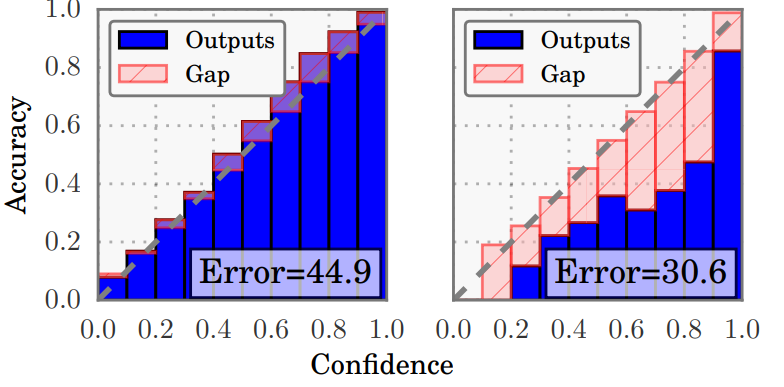
\includegraphics[width=0.7\linewidth]{./Figures/reliab.png}
	\caption{Figure 1 from \textcite{guo2017calibration}: Confidence vs accuracy for a 5-layer LeNet (left) and a 110-layer ResNet (right).
		Gap shows miscalibration.
	For example, on the right hand side, we see that on average, an $80 \%$ output confidence does not correspond to $80 \%$ accuracy, but less.}
	\label{fig:reliab}
\end{figure} 

\paragraph{Other metrics:}
The expected calibration error is a weighted average of the calibration gaps $|acc(B_m)-conf(B_m)|$ over the interval bins and the maximum calibration error is the maximum value of $|acc(B_m)-conf(B_m)|$.
The negative log likelihood on unseen data is also a metric of calibration. 

\paragraph{Post-hoc recalibration:}\label{sec:posthoc}
Consider a binary classification NN and a calibration set of size $n$ used for recalibration of the NN (this set could be the same as the validation set used for tuning hyperparameters).
One way to recalibrate the predicted confidence is to divide the confidence axis into $M$ interval bins and assign each prediction $\hat{p}_i$ into the corresponding bin. 
Then a calibrated score $\theta_m$ is assigned to each bin. 
In other words, if $\hat{p}_i$ is assigned to bin $m$ then the corresponding prediction is no longer $\hat{p}_i$, but $\hat{q}_i=\theta_m$.
Next, consider that $M$ and the bin boundaries $a_m$ for every $m$ are fixed. 
The optimal values of the calibrated scores $\theta_m$ can be obtained by minimizing the bin-wise squared loss, i.e.,
\begin{equation}
\underset{\theta_1,\dots,\theta_m}{\mathrm{min}}~\sum_{m=1}^{M}\sum_{i=1}^{n} \textbf{1}(a_m \leq \hat{p}_i < a_{m+1})(\theta_m-y_i)^2
\end{equation}
This is called histogram binning. 
Further, isotonic regression pertains to optimizing also $M$ and the bin boundaries. 

Another approach is Platt scaling, according to which the recalibrated predictions become $\hat{q}_i=\sigma(az_i+b)$, where $z_i$ is the nonprobabilistic prediction of the classifier (before it is passed through the sigmoid function) and $a$, $b$ are parameters to be optimized using the negative log likelihood loss over the calibration set (for fixed weights).

An equivalent way to view the above techniques, as described in \textcite{kuleshov2018accurate}, is as approximators of the accuracy for given values of confidence; i.e., as approximators of $P(Y = 1 | f_{\cH}(X) = p)$ in Eq.~\eqref{classcalibr}. 
Given a value of confidence $\hat{p}_i$ from the NN, the recalibrator (trained on the calibration set) provides an estimate of the accuracy $P(Y = 1 | f_{\cH}(X) = \hat{p}_i)$; this becomes the final output $\hat{q}_i$. 
Following the recalibration step, the NN is \textit{on average calibrated}.

The above techniques can be extended to multi-class classification (\cite{guo2017calibration}). 
An interesting extension of Platt scaling uses a single ``temperature'' parameter $T>0$ for all classes. 
In this regard, the confidence prediction becomes 
\begin{equation}
\hat{q}_i = \underset{k}{\mathrm{max}}~\sigma_{SM}(\boldsymbol{z}_i/T)^{(k)}
\end{equation}
where $\boldsymbol{z}_i$ is the logit vector and $\sigma_{SM}$ denotes the softmax function.
The optimal $T$ is obtained with respect to the negative log likelihood loss over the calibration set. 
Also, temperature scaling does not change the maximum of the softmax function, i.e., the predicted class will be the same, only the confidence changes. 
Therefore, temperature scaling does not affect the model accuracy. 
\textcite{guo2017calibration} notes that for remedying miscalibration, temperature scaling is the simplest, fastest, and most straightforward of the methods they considered, and surprisingly is often the most effective.
Motivated by the results of \textcite{guo2017calibration}, \textcite{wenzel2020how} and \textcite{wilson2020bayesian} further studied the effects of temperature scaling.

\paragraph{Calibration via epistemic uncertainty:}
As noted in \textcite{ovadia2019can}, in practice, once a model is deployed the distribution over observed data may shift and eventually be very different from the original training data distribution.
In that case, we would like the predictions to indicate that a model ``knows what it does not know'' due to the inputs straying away from the training data distribution (see Section~\ref{sec:quality}).
In this regard, \textcite{ovadia2019can} has found that post-hoc calibration with temperature scaling leads to well-calibrated uncertainty on the independent and identically distributed (i.i.d.) test set and for small values of dataset shift, but is significantly outperformed by methods that take epistemic uncertainty into account as the shift increases.

In general, miscalibration happens because we ignore epistemic uncertainty, i.e., the fact that we are not sure if we have selected the correct model parameters. 
If epistemic uncertainty is large, the models implied by the posterior disagree on a test point and including other models as well makes the confidence decrease.
Incorporating epistemic uncertainty by accounting for more than one plausible models (parameter settings) via the BMA of Eq.~\eqref{new_data_4} is the focus of these notes. 

\subsubsection{Calibration in the regression setting}\label{sec:calib}
For regression, the NN outputs a single value with no uncertainty, i.e., it is $100 \%$ confident. 
Calibration in this context relates to taking into account other models as well and thus admitting some uncertainty in the output.
A well-calibrated network should predict with high uncertainty far from data, as well as in regions between separated clusters of observations (see Section~\ref{sec:quality}).
For example, in Fig.~\ref{fig:pointvsbnn}, the probabilistic model is more calibrated than the standard NN: for a test point (shown with red) far from the training data (left of the dashed blue line) the standard NN confidently predicts a value, whereas the probabilistic model predicts a similar value but with high uncertainty.
This test point far from the training data is called out-of-distribution datapoint.
\begin{figure}
	\centering
	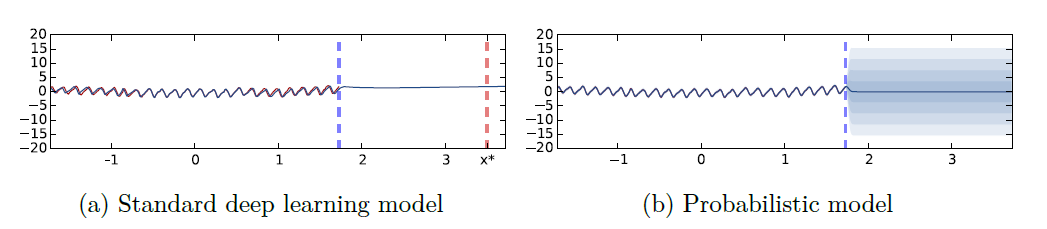
\includegraphics[width=0.9\linewidth]{./Figures/pointvsbnn.png}
	\caption{Figure 1.2 from \textcite{gal2016uncertainty}: Standard NN vs a probabilistic model trained on data to the left of the blue dashed line.
		Different shades of blue represent half a standard deviation. Marked with a dashed red line is a point far away from the data: standard deep learning models confidently predict an unreasonable value for the point; the probabilistic model predicts an unreasonable value as well but with the additional information that the model is uncertain about its prediction.}
	\label{fig:pointvsbnn}
\end{figure} 

Finally, even if epistemic uncertainty is taken into account by using a BNN, the obtained confidence \textit{may still be miscalibrated}. 
BNN uncertainty quality as well as recalibration methods are discussed in Section~\ref{sec:quality}.
%See \textcite{wilson2020bayesian} for tempering techniques for further calibration and discussions in \textcite{yao2019quality} and \textcite{hafner2018reliable}. 

\subsubsection{Accuracy}

Accuracy refers to the correctness of the NN output.
According to \textcite{wilson2020bayesian}, the MAP approximation of Eq.~\eqref{new_data_map} (as opposed to using the exact Eq.~\eqref{new_data_4}) is reasonable only if $p(\bw|\cD,\cH)$ is peaked around $\hat{\bw}$ and also $p(y^*|x^*, \bw, \cH)$ does not vary much where the mass of $p(\bw|\cD,\cH)$ is. 
However, modern NNs are usually highly underspecified by the available data, and therefore have diffuse likelihoods, not strongly favoring any one setting of parameters.
Further, different settings of parameters correspond to a diverse variety of compelling hypotheses for the data (\cite{garipov2018loss}). 

Therefore, this is a setting that can benefit from using a BMA. 
According to \textcite{wilson2020bayesian}, even a Gaussian approximation to the posterior (Laplace approximation; see Section~\ref{sec:laplace}) is preferable to the MAP approximation. 

\section{Components of Bayesian deep learning}\label{sec:components}

As discussed in \textcite{blei2014build}, building and computing with Bayesian models is an iterative process. 
This process involves building a model (architecture and priors in BNNs), inferring model parameters (posterior distribution), and criticizing the model (optimizing hyperparameters, comparing different models, re-building the model).
This process is briefly discussed in this section.

\subsection{Model building}

\subsubsection{Stochastic NNs and BNNs}\label{sec:stochastic_NNs}
As described in \textcite{jospin2020handson}, stochastic NNs are built by introducing stochastic components into a NN. 
The stochastic components can either be stochastic activations  where only a set of weights along with a probability distribution for the activation is learned (Fig.~\ref{fig:BNNs}-left), or stochastic weights where a probability distribution over the weights is learned (Fig.~\ref{fig:BNNs}-right).
A BNN is a stochastic NN trained using Bayesian inference.
In these notes, BNNs with stochastic weights are considered. 

A BNN can be easily understood through its generative process; i.e., the way the stochastic components interact with the functional form of the NN for producing observations. 
Specifically, for a regression BNN, the data generating process involves drawing a parameter vector from the prior and then for each datapoint drawing an observation from a Gaussian distribution with mean the output of the NN (with the drawn parameter vector) and a pre-specified variance.
Inference refers, thus, to the opposite process: having collected a set of datapoints we seek to infer what the drawn parameter vector could have been.

As noted by \textcite{wilson2020bayesian}, for building a model with satisfactory generalization properties what matters is the distribution over functions (functional prior) 
\begin{equation}\label{functional_prior}
	p(f_{\cH}(x)) = \int f_{\cH}(x;\bw) p(\bw|\cH) d\bw
\end{equation}
that is induced by both the functional form of the model $f_{\cH}(x;\bw)$ and the parameter prior $p(\bw|\cH)$.
In this regard, $p(f_{\cH}(x))$ depends on the selected network architecture, the noise model, the priors, the grouping of parameters with different priors for each group (see \cite{neal1995bayesian} p. 77) and the values of the hyperparameters.
In Sections~\ref{sec:GP_limit}-\ref{sec:functional}, how the parameter prior with the functional form interact is briefly demonstrated.

\begin{figure}
	\centering
	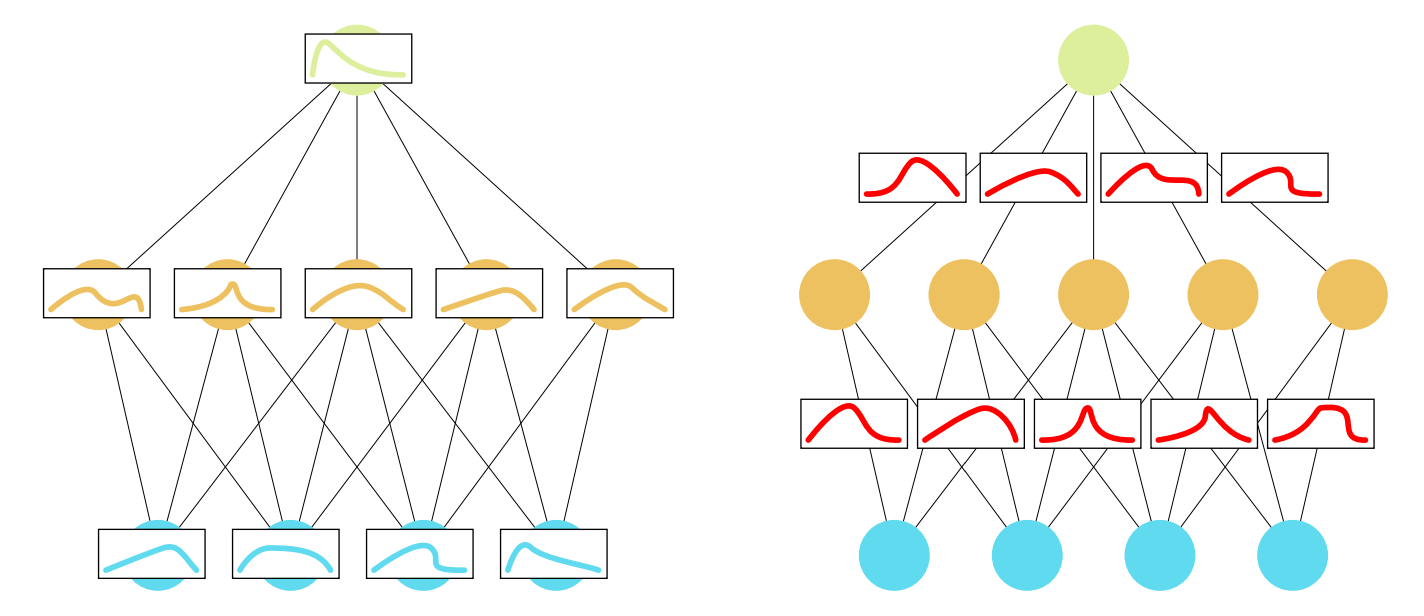
\includegraphics[width=0.9\linewidth]{./Figures/BNNs.png}
	\caption{Figure 3 from \textcite{jospin2020handson}: The stochastic components can either be stochastic activations  where only a set of weights along with a probability distribution for the activation is learned (left) or stochastic weights where a probability distribution over the weights is learned (right).}
	\label{fig:BNNs}
\end{figure} 

\subsubsection{Gaussian process limit}\label{sec:GP_limit}

It has been shown in \textcite{neal1995bayesian} that under certain conditions, placing a Gaussian prior on $\bw$ and taking the number of hidden units of a single-layer NN to infinity results in the NN becoming a Gaussian process (GP). 
This is based on the central limit theorem (CLT).
In this regard, the NN induces some covariance function that can be used with the convenient theory of GPs for exact Bayesian inference.  
Note that besides its importance, the discussion in \textcite{neal1995bayesian} is limited to only proving the above result. 
\textcite{neal1995bayesian} did not eventually obtain the induced covariance function nor did he use this limit in his calculations; he instead used large but finite NNs and obtained his results with approximate inference (see Section~\ref{sec:hmc}). 

\textbf{Historical note:} \textcite{williams1997computing} computes the covariance of the infinite network; he actually obtains a neural-net-induced GP (NNGP) for the error and the Gaussian activation functions and performs exact Bayesian inference.
\textcite{lee2017deep} computes the covariance function recursively for other activation functions and coins the term NNGP.
\textcite{lee2017deep} also extends the result of \textcite{neal1995bayesian} to deep NNs.
\textcite{pang2019neuralnetinduced} compares NNGPs with GPs and finite NNs, and notes that NNGPs can be more flexible than NN and do not suffer from overfitting because they are Bayesian.
Nevertheless, they can address only linear or linearized problems in the context of physics-informed NNs.

However, the aforementioned infinite limit does not imply that GPs can replace NNs (see discussion in \cite{mackay1998introduction} p. 30).
As \textcite{neal1995bayesian} puts it, in the infinite limit the contributions of individual units are all negligible, and consequently, these units do not represent hidden features that capture important aspects of the data.
According to \textcite{nalisnick2018priors}, for finite NNs there are ``jumps'' in the regression line, meaning that the function can change drastically depending on which hidden units are active (see Fig.~\ref{fig:BNNs_with_priors}a-left).
On the other hand, for infinite width NNs the regression line becomes Brownian motion: it wanders according to very small, independent increments (see Fig.~\ref{fig:BNNs_with_priors}a-right).
Also, according to \textcite{matthews2018gaussian}, a GP with a fixed kernel does not use a learned hierarchical representation. 
Such representations are widely regarded to be essential to the success of deep learning. 
Instead only a few hyperparameters are learned and it seems unlikely this could offer the same benefits as full representation learning. 

The practical implications of the work of \textcite{matthews2018gaussian} are worth noting. 
Specifically, \textcite{matthews2018gaussian} has proved the convergence of certain sequences of \textit{finite} fully connected networks with more than one hidden layer to GPs.
The authors note that it seems likely that some experiments in the literature studied under the banner of Bayesian deep learning would have given very similar results to a GP with the correct kernel.
As a result, they propose that the Bayesian deep learning community routinely compare their results to GPs with the kernels studied in \textcite{matthews2018gaussian}. 
According to \textcite{nalisnick2018priors}, this tendency can be a good thing for GP users as it means that BNNs can be used as plug-in approximations for GPs.  
Swapping a GP for a BNN results in considerable computational savings for large datasets since the user is trading the GP’s $\cO(N^3)$ cost of matrix inversions and determinants for the BNN’s $\cO(N)$ training data dependence (see, for example, \cite{flam-shepherd2017mapping} where a matching between the GP prior is attempted by using a BNN and minimizing a KL divergence; more information in Section~\ref{sec:functional}).

In summary, even NNs with discrete weights will converge to GPs via the Lyapunov CLT if the hidden units are real-valued (\cite{matthews2018gaussian}).
If the full capabilities of BNNs are required, one has to make sure that one or more of the conditions discussed in \textcite{matthews2018gaussian} are not satisfied. 
This can be done by considering CLT-breaking priors discussed in the next section (see \cite{nalisnick2018priors} for an excellent review and discussions).

\begin{figure}
	\centering
	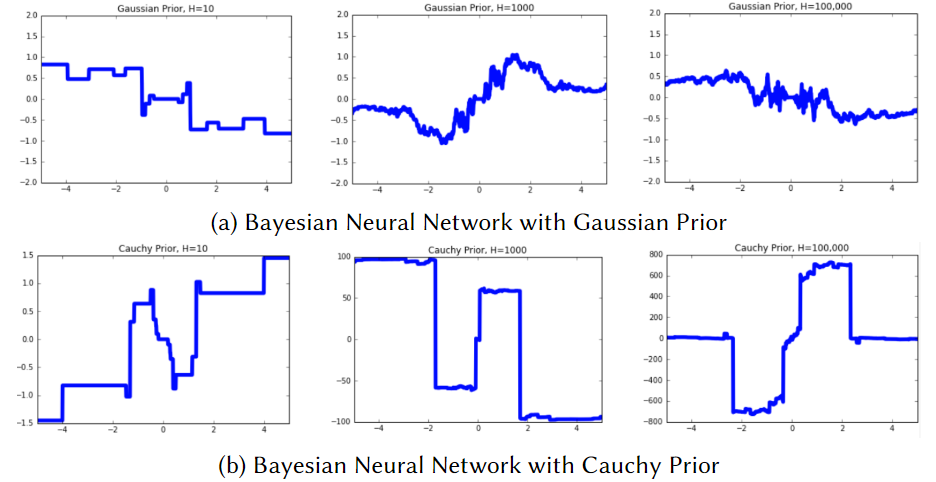
\includegraphics[width=1\linewidth]{./Figures/BNNs_with_priors.png}
	\caption{Figure 3.1 from \textcite{nalisnick2018priors}: GP behavior of BNNs.}
	\label{fig:BNNs_with_priors}
\end{figure} 

\subsubsection{Parameter priors}

\paragraph{Noninformative/objective priors:} These priors aim to inject as little information as possible into the inference procedure. 
An objective prior is one that has some formal invariance property. 
The two best known examples of objective priors are Jeffreys' non-informative priors and, their extension, reference priors, which are both invariant to model reparametrization.
Reference priors are model-dependent and notoriously difficult to derive for complicated models (\cite{simpson2015penalising}). 
According to \textcite{nalisnick2018priors}, the mathematical rigor that makes objective priors attractive also makes their use problematic: their derivation is difficult for all but the simplest models. 
In this regard, \textcite{nalisnick2018priors} proposes approximate constructions of such priors. 

\paragraph{Weakly informative priors:} Between objective and expert priors lies the realm of ``weakly informative'' priors. 
These priors are constructed by recognizing that while you usually do not have strong prior information about the value of a parameter, it is rare to be completely ignorant. 
This use of weak prior knowledge is often sufficient to regularize the extreme inferences that can be obtained using maximum likelihood (\cite{simpson2015penalising}).

Such priors are typically written in a hierarchical form by assuming they are drawn from a hyperprior (Section~\ref{sec:hyperpriors}). 
Typically, a Gaussian scale mixture is considered; i.e., the parameters are drawn from a Gaussian with variance drawn from some hyperprior. 
In this regard, we obtain a Student-t prior by using a Gaussian distribution with scale drawn from an inverse Gamma hyperprior, a Laplace prior by using an exponential hyperprior, and a horseshoe prior by using a half-Cauchy hyperprior (the Cauchy distribution restricted to the positive real numbers). 

A Gaussian prior for the parameters is a typical and reasonable choice because the zero-centering induces shrinkage and the Gaussian assumption implies smoothness (\cite{nalisnick2018priors}). 
However, as discussed in Section~\ref{sec:GP_limit}, even finite-width BNNs may behave like GPs. 

According to \textcite{nalisnick2018priors}, one way to break the CLT is to draw the NN weights from a distribution with infinite variance; such as from a member of the symmetric stable family with index less than two.  
These distributions have heavy, sub-exponential tails, which allows ``some of the hidden units in an infinite network [to] have output weights of significant size, allowing them to represent hidden features'' (\cite{neal1995bayesian}). 
Unfortunately, heavy-tailed distributions are not easy to work with analytically or computationally.  
The Cauchy, for instance, does not have finite moments of any order.  \textcite{neal1995bayesian} recommends the Student-t distribution as a compromise, which is CLT-breaking when its degrees of freedom parameter is less than two. 
In Fig.~\ref{fig:BNNs_with_priors}b taken from \textcite{nalisnick2018priors}, we see that when a Cauchy prior is used the regression line exhibits \textit{large jumps} even for large widths, which means that the regression function is still dependent on which hidden units are active.

Another choice is the Laplace prior which, due to its dependence on the absolute value of the weights, reflects the symmetry of NNs with respect to the signs of the weights (\cite{williams1995bayesian}). 
Laplace priors may not provide enough regularization under fully Bayesian treatments of NNs. 
Note that Laplace priors do not induce the same amount of useful sparsity in their posteriors as is found in their MAP estimates.

Next, the horseshoe prior has no closed-form marginal expression, but it can be easily plotted. 
This prior allows the NN weights to grow large, like the Student-t, but has fierce shrinkage near zero.
These facts make the horseshoe prior a stronger regularizer than the Gaussian, Laplacian, and Student-t densities.

There are also priors without a hierarchical form. 
For example, a variational-inference-based analysis lead \textcite{kingma2015variational} to find that the log-uniform distribution is the Bayesian prior that best mimics the dropout mechanism. 
It is similar to the horseshoe prior but has flatter tails and better sparsity inducing behavior.
See Fig.~\ref{fig:priors} for density comparisons. 

\begin{figure}
	\centering
	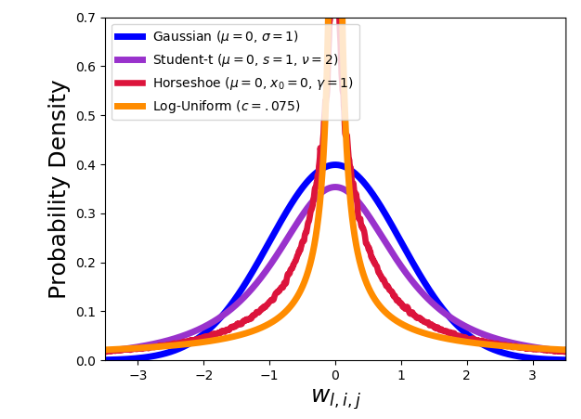
\includegraphics[width=0.7\linewidth]{./Figures/priors.png}
	\caption{Figure 3.2a from \textcite{nalisnick2018priors}: Heavy-tailed priors.}
	\label{fig:priors}
\end{figure} 

\subsubsection{Functional priors}\label{sec:functional}
As noted in \textcite{wilson2020bayesian}, although it is popular recently to build directly function-space BNN priors (see $p(f_{\cH}(x))$ in Eq.~\eqref{functional_prior}), if we contrive parameter priors $p(\bw)$ to induce distributions over functions $p(f_{\cH}(x))$ that resemble familiar models we could be doing the same mistake as when replacing BNNs by GPs. 
NNs are useful as their own model class precisely because they have different inductive biases from other models.
Nevertheless, some techniques pertaining to constructing functional priors are presented in this section.

\textcite{hafner2018noise} proposes an implicit functional prior by constructing a data prior.
In other words, this prior favors functions that are similar to the data. 
The authors also perform active learning by selecting new datapoints that maximize the expected information gain. 
Their prior encourages the BNN to assign high uncertainty (as it should) to datapoints that are out of the distribution that generated the training data (see also Section~\ref{sec:quality}).
Specifically, a prior $\cP$ is constructed according to which each training datapoint is modeled as
\begin{equation}
	p(x_i,y_i|\cP) = p(x_i|\cP)p(y_i|x_i,\cP)
\end{equation}
Next, for points $\tilde{x}$ that are perturbations of the training points, the prior gives
\begin{equation}
p(\tilde{x}|\cP) = \frac{1}{N}\sum_{i=1}^{N}\cN(\tilde{x}-x_i|0,\sigma_x^2)
\end{equation}
and 
\begin{equation}
p(\tilde{y}|\tilde{x},\cP) = \cN(y,\sigma_y^2)
\end{equation}
where $\cN$ denotes a Gaussian distribution and $\sigma_x^2, \sigma_y^2$ are tunable parameters.
Further, $y$ is not clearly defined in the manuscript but its purpose is recovering true labels/values from perturbed inputs $\tilde{x}$.
By introducing a data prior, a functional prior is implicitly introduced. 
To see this, consider the marginal likelihood of a datapoint given as
\begin{equation}
	p(y|x) = \int p(y|x,\bw,\cH)p(\bw|\tilde{x},\tilde{y},\cH)p(\tilde{x},\tilde{y}|\cP)d\bw d\tilde{x}d\tilde{y}
\end{equation}
Clearly, $p(\tilde{x},\tilde{y}|\cP)$ induces a parameter prior $p(\bw|\tilde{x},\tilde{y},\cH)$ which in turn induces a functional prior $p(y|x)$. 
Finally, training is performed by variational inference where instead of penalizing the posterior for being far from the parameter prior, the posterior predictive
\begin{equation}\label{posterior_predictive}
	q(f_{\cH}(\tilde{x}))=\int f_{\cH}(\tilde{x};\bw)q_{\bth}(\bw) d\bw 
\end{equation}
defined using the approximate parameter posterior $q_{\bth}(\bw)$, is penalized for being far from the data prior.
Note the similarity of Eq.~\eqref{posterior_predictive} with Eq.~\eqref{new_data_4} and see also Section~\ref{sec:vi} for more information on variational inference.

Next, \textcite{flam-shepherd2017mapping} trains a BNN to mimic the behavior of a GP prior, by encoding properties of GP priors into BNN weight priors, and performs standard variational inference in the weight space. 
On the contrary, \textcite{sun2019functional} have proposed functional variational BNNs for which variational inference is performed directly in the function space and have shown how to also handle functional priors without tractable marginal densities $p(f_{\cH})$; i.e., functional priors other than GPs and Student-t processes. For example, they consider piecewise constant functions and piecewise linear functions. 
Further, \textcite{ma2019variational} have introduced variational implicit processes which, in a sense, are the reverse of functional variational BNNs. 
A GP is trained to mimic the behavior of the BNN functional prior and the resulting GP is used for exact Bayesian inference. 

Functional neural processes, introduced in \textcite{louizos2019functional}, posit distributions over functions by embedding the dataset into a latent space and constructing a dependency graph among the latent embeddings; recall that in GPs a correlation structure encoded in the covariance matrix measures the similarity between inputs.
Finally, \textcite{yang2019outputconstrained} proposes a way of enforcing expert knowledge into the BNN prior in the form of constraints restricting where the function should or should not be. 

\subsection{Approximate inference}\label{sec:inference}
Obtaining the posterior exactly via Eqs.~\eqref{posterior_2} or \eqref{posterior_params} is computationally and analytically intractable. 
In this regard, approximate inference refers to approximating the posterior by another distribution and/or obtaining samples from the posterior. 
As shown in Section~\ref{sec:MAP}, the MAP estimate of Eq.~\eqref{map_p} (standard training of NNs) can be seen as an approximate inference technique. 
However, being a point estimate, the MAP estimate is not Bayesian. 
In this section, the most widely used Bayesian (or not) approximate inference techniques are briefly reviewed. 

\subsubsection{Monte Carlo estimation}\label{sec:mc} 
According to the law of large numbers, for i.i.d. samples $\hat{w}_1,\dots,\hat{w}_M$ with mean $\mu$ the condition 
\begin{equation}
	\lim\limits_{M\to \infty} P\left(\bigg|\frac{\sum_{j=1}^M\hat{w}_j}{M}-\mu\bigg|\geq b \right) = 0
\end{equation}
is satisfied for any positive $b$.
Similarly, 
\begin{equation}
\lim\limits_{M\to \infty} P\left(\bigg|\frac{\sum_{j=1}^Mg(\hat{w}_j)}{M}-\mathbb{E}_w[g(w)]\bigg|\geq b \right) = 0
\end{equation}
As a result, the predictive distribution of Eq.~\eqref{new_data} can be approximated by a Monte Carlo (MC) estimate as
\begin{equation}\label{new_data_mc}
p(y^*|x^*, \cD, \cH) = \mathbb{E}_{\bw|\cD}[p(y^*|x^*, \bw,\cD, \cH)] \approx \frac{1}{M}\sum_{j=1}^Mp(y^*|x^*, \hat{\bw}_j,\cD, \cH)
\end{equation}
where $\{\hat{\bw}_j\}_{j=1}^M$ are samples from the posterior $p(\bw|\cD,\cH)$.

If also hyperparameters are included as in Eq.~\eqref{new_data_hypers}, $p(y^*|x^*, \cD, \cH)$ can be approximated as 
\begin{equation}\label{new_data_mc_2}
p(y^*|x^*, \cD, \cH) = \mathbb{E}_{\bw,\alpha,\beta|\cD}[p(y^*|x^*, \bw,\cD, \beta,\cH)] \approx \frac{1}{M}\sum_{j=1}^Mp(y^*|x^*, \hat{\bw}_j,\hat{\beta}_j,\cD, \cH)
\end{equation}
where  $\{\hat{\bw}_j,\hat{\beta}_j\}_{j=1}^M$ are samples from the posterior $p(\bw,\alpha,\beta|\cD,\cH)$ ($\alpha$ is used to draw values for $\bw$).
If, instead, the hyperparameters are optimized (see Section~\ref{sec:evidence}), then 
$p(y^*|x^*, \cD, \cH)$ can be approximated as 
\begin{equation}\label{new_data_mc_3}
p(y^*|x^*, \cD, \cH) = \mathbb{E}_{\bw|\cD,\hat{\alpha},\hat{\beta}}[p(y^*|x^*, \bw,\cD, \hat{\beta},\cH)] \approx \frac{1}{M}\sum_{j=1}^Mp(y^*|x^*, \hat{\bw}_j,\hat{\beta},\cD, \cH)
\end{equation}
where $\{\hat{\bw}_j\}_{j=1}^M$ are samples from the posterior $p(\bw|\cD,\hat{\alpha},\cH)$ and $\hat{\alpha}$, $\hat{\beta}$ are the optimal hyperparameters.

Therefore, using one of the above MC estimates transforms the original problem into a sampling problem: we need to draw independent samples $\{\hat{\bw}_j\}_{j=1}^M$ from the posterior. 
Drawing independent samples is not straightforward. 
Fortunately, the above MC estimates (typically with slower convergence) still hold for moderately dependent samples from the posterior (see \cite{neal1995bayesian} p. 27).

Finally, note that, instead of Eq.~\eqref{new_data}, an approximation of Eq.~\eqref{new_data_2} or \eqref{new_data_4} may be required. 
Thus, to make the formulation more general, the more diverse problem of approximating 
\begin{equation}\label{mean_g}
	\mathbb{E}_{\bw|\cD}[g(\bw)] = \int g(\bw)p(\bw|\cD,\cH)d\bw
\end{equation}
is considered herein. 
Typically, the posterior is written as
\begin{equation}\label{canonical}
p(\bw|\cD,\cH) = \frac{f(\bw)}{Z} = \frac{\exp(-\cL(\bw))}{Z}
\end{equation}
where $f(\bw) = p(\cD|\bw,\cH)p(\bw|\cH)$ and $Z$ is a normalization constant. 
Therefore, Eq.~\eqref{mean_g} can also be expressed as
\begin{equation}\label{mean_g_2}
\mathbb{E}_{\bw|\cD}[g(\bw)] = \frac{\int g(\bw)f(\bw)d\bw}{\int f(\bw)d\bw}
\end{equation}
%and approximated as
%\begin{equation}\label{mean_g_2_mc}
%\mathbb{E}[g(\bw)] \approx \frac{\sum_{j=1}^M g(\hat{\bw}_j)f(\hat{\bw}_j)}{\sum_{j=1}^M f(\hat{\bw}_j)}
%\end{equation}
%where samples are drawn from the un-normalized $f(\bw)$.

MC methods have been widely used in statistical physics. 
For this reason, the terminology originating from their use in statistical physics often accompanies them even when used in domains other than physics. 
For example, the distribution of Eq.~\eqref{canonical} is called canonical distribution over microstates $\bw$, $\cL(\bw)$ is the energy of the system defined for each microstate $\bw$, and $Z$, the normalization constant, is known as the partition function. 
See \textcite{neal1993probabilistic}, Section~2.4, for more information on this correspondence.

\subsubsection{Rejection and importance sampling}
This section follows closely the review paper \textcite{neal1993probabilistic}.
Suppose that there is a function $q(\bw)$, that is proportional to a density easy to sample from, and that there is also a constant $c$ such that $f(\bw)<c q(\bw)$ is satisfied for any $\bw$.
Then, for obtaining samples from $f(\bw)$ we can generate a candidate sample $\bw^*$ from $q(\bw)$ and accept it with probability $p=f(\bw^*)/cq(\bw^*)$. 
This is known as rejection sampling and is equivalent to drawing also some $u$ from a uniform distribution in $[0,1)$ and accepting $\bw^*$ if $u<p$.
Unfortunately, it is almost impossible to find an appropriate $q(\bw)$ with small $c$.

Suppose, next, that there is a density $q(\bw)$ (not necessarily normalized) that is nonzero where $f(\bw)$ is nonzero. 
Then, following Eq.~\eqref{mean_g_2}, $\mathbb{E}_{\bw|\cD}[g(\bw)]$ can be written as
\begin{equation}\label{importance}
\mathbb{E}_{\bw|\cD}[g(\bw)] = \frac{\int g(\bw)\frac{f(\bw)}{q(\bw)}q(\bw)d\bw}{\int \frac{f(\bw)}{q(\bw)}q(\bw)d\bw} = \frac{\mathbb{E}_{\bw\sim q}[g(\bw)\frac{f(\bw)}{q(\bw)}]}{\mathbb{E}_{\bw\sim q}[\frac{f(\bw)}{q(\bw)}]}
\end{equation}
which can be approximated in a similar way as Eq.~\eqref{new_data_mc} (see Eq.~(3.6) in \cite{neal1993probabilistic}).
If $q(\bw)$ is a good approximation of $f(\bw)$ then an MC estimate of Eq.~\eqref{importance} will be a good estimate of $\mathbb{E}_{\bw|\cD}[g(\bw)]$. 
However, guessing such a density $q(\bw)$ is not easy and thus, this technique, known as simple importance sampling, is not applicable in the context of deep learning. 

\subsubsection{Markov chain sampling}
This section follows closely the review paper \textcite{neal1993probabilistic} and the more compact summary in \textcite{neal1995bayesian}.

\paragraph{Markov chains:}
A sequence of dependent $\bw$ values can be generated using a Markov chain with $p(\bw|\cD,\cH)$ as its invariant (stationary) distribution; this idea defines a family of techniques known as Markov chain Monte Carlo (MCMC). 
The first state of the chain is $\bw^{(1)}$ and it has some initial distribution. 
A transition probability is also defined for each state $t$ denoted by $T_t(\bw^{(t+1)}|\bw^{(t)})$. 
If $T_t$ does not depend on $t$ then the Markov chain is called homogeneous with transition probability $T$. 
An invariant or stationary distribution $q$ is one for which if $\bw^{(t)}$ has distribution $q$, then any $\bw^{(t')}$ with $t'>t$ will also have distribution $q$.
An ergodic Markov chain has a unique invariant distribution called equilibrium distribution. 
Whatever the initial state $\bw^{(1)}$ is, the same equilibrium distribution will be reached in stationarity. 

Therefore, if we can construct an ergodic Markov chain with equilibrium distribution $q(\bw)=p(\bw|\cD,\cH)$, then we can sample from $p(\bw|\cD,\cH)$ by sampling from $q(\bw)$; this can be performed by simulating the Markov chain and discarding some ``burn-in'' states until it reaches equilibrium. 
After we sample one state then we can start over the Markov chain with the sampled state as the initial state.
Due to ergodicity, whatever the sampled state was, after a few steps the equilibrium distribution $q$ will be reached again. 
We can thus \textit{resample from the same realization} after some ``lag'' steps. 

One way to construct an ergodic Markov chain is by applying a set of base transitions $B_1,\dots,B_k$ in turn (e.g., by changing only a subset of the dimensions of $\bw^{(t)}$ in each transition). 
In this regard, $q$ needs to remain invariant with respect to each transition, so that it remains invariant with respect to the overall transition $T=B_1\cdots B_k$, where a center dot denotes sequential transitions.
This is utilized, for instance, in Gibbs sampling.

As an illustrative example, consider the homogeneous Markov chain that starts from state $0$ and moves left or right $\pm 1$ with probability $1/4$ and stays at the same state with probability $1/2$. 
Suppose also that it is confined in the finite space $\{-5,\dots,5\}$. 
This confined random walk is ergodic with the uniform distribution as its equilibrium distribution. 
As a result, a sample from the uniform distribution can be obtained by simulating the random walk for some sufficiently large number of iterations. 
This is depicted in Fig.~\ref{fig:mc} for two different numbers of iterations. 
\begin{figure}
	\centering
	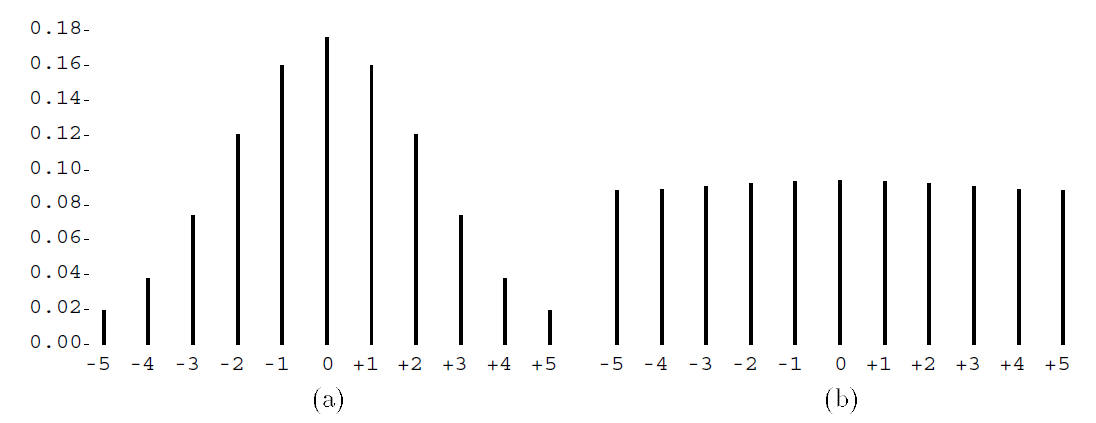
\includegraphics[width=0.85\linewidth]{./Figures/mc.png}
	\caption{Figure 3.2 from \textcite{neal1993probabilistic}: Distribution of confined random walk states (a) after $10$ iterations and (b) after $100$ iterations. 
	A sample from the uniform distribution can be obtained by simulating the random walk for some sufficiently large number of iterations.}
	\label{fig:mc}
\end{figure} 

\paragraph{Gibbs sampling:}\label{sec:gibbs}
Possibly the simplest Markov chain-based sampling scheme is Gibbs sampling. 
For a $k$-dimensional $\bw$ vector, $k$ transitions $B_1,\dots,B_k$ are considered; in each one only one dimension of the $t$-th state $\bw^{(t)}$ is changed using the conditional distribution (under $p(\bw|\cD,\cH)$) of each dimension given the current values of all the rest.
This technique is widely used in the context of latent variable models (e.g., \cite{blei2014build}), but in deep learning the conditional distributions under the posterior are typically not available. 

\paragraph{Metropolis algorithm:}
A new state $\bw^{(t+1)}$ is generated from $\bw^{(t)}$ by first generating a candidate state using a proposal distribution $S(\bw^*|\bw^{(t)})$ and then deciding whether to accept the candidate or not. 
If it is not accepted, $\bw^{(t+1)}$ is taken to be $\bw^{(t)}$.
The steps, thus, are
\begin{enumerate}
	\item generate $\bw^*$ from some proposal distribution $S(\bw^*|\bw^{(t)})$
	\item if $\frac{p(\bw^*|\cD,\cH)}{p(\bw^{(t)}|\cD,\cH)} = \exp(-\cL(\bw^*)+\cL(\bw^{(t)}))\geq 1$, then accept $\bw^*$, otherwise accept $\bw^*$ with probability $p = \exp(-\cL(\bw^*)+\cL(\bw^{(t)}))$
	\item if $\bw^*$ is accepted, then set $\bw^{(t+1)} = \bw^*$, otherwise set $\bw^{(t+1)} = \bw^{(t)}$. 
\end{enumerate}
Although the form of the acceptance probability can be different than the one in Step~2, acceptance or rejection of the candidate state is typically based on the change of ``energy'' $\cL$.
The proposal distribution $S(\bw^*|\bw^{(t)})$, among many choices, can be a Gaussian distribution centered at $\bw^{(t)}$. 

\paragraph{The stochastic dynamics method:}
The canonical distribution for the ``position'' variable $\bw$ of the corresponding to statistical inference physical system is defined in Eq.~\eqref{canonical}.
For formulating the stochastic dynamics method, a ``momentum'' variable $\bp$ is also introduced for which there is one-to-one correspondence with the components of $\bw$.
The canonical distribution for the phase space of $\bw$ and $\bp$ is defined as 
\begin{equation}
p(\bw,\bp) \propto \exp(-H(\bw,\bp))
\end{equation}
where $H(\bw,\bp) = \cL(\bw) + K(\bp)$, with $K$ denoting the ``kinetic'' energy, is the total energy of the system and is known as the Hamiltonian function. 
In this regard, $\bw$ and $\bp$ are independent, i.e., the marginal of $\bw$ under $p(\bw,\bp)$ is the same as the one we seek to sample from. 
Thus, a Markov chain that converges to $p(\bw,\bp)$ can be constructed and $\bw$ samples can be collected by sampling from $p(\bw,\bp)$ and discarding the $\bp$ samples.

In the stochastic dynamics method there are two sub-tasks: 1) sampling states $(\bw,\bp)$ with fixed energy $H$, and 2) sampling states with different values of $H$. 
Loosely speaking, in the first task we obtain different samples of $\bw$ by simply following the Hamiltonian dynamics of the system without visiting states of different probability, and in the second task we visit states with different probability by changing only the state of $\bp$, which is straightforward. 
Task 1 is done by simulating the Hamiltonian dynamics of the system, in which the state $(\bw,\bp)$ evolves in fictitious time $\tau$. 
It can be shown that $H$ stays the same and thus, $p(\bw,\bp)$ is invariant with respect to transitions related to following a trajectory based on the Hamiltonian dynamics equations. 
In many cases these transitions will eventually explore the whole range of phase space with fixed $H$.
Task 2 is done by Gibbs sampling updates of the momentum via its density which is proportional to $\exp(-K(\bp))$. 
If, for example, $K(\bp)$ is taken to be $K(\bp) = \norm{\bp}_2^2/2$, then the conditional distributions required by Gibbs sampling are readily available (the components of $\bp$ have independent Gaussian distributions). 

In practice, Hamiltonian dynamics are simulated by some discretization using finite time steps (e.g., leapfrog method). 
To follow the dynamics for some period of fictitious time $\Delta \tau$ (see \cite{neal1993probabilistic} for selecting $\Delta \tau$), $T = \Delta \tau/\epsilon$ iterations are applied, with $\epsilon$ the time step. 
Using the leapfrog method, $H$ does not stay exactly the same; MC estimates obtained via the stochastic dynamics method will have some systematic error that goes to zero as $\epsilon$ goes to zero. 
This systematic error is eliminated in the hybrid MC (HMC; also known as Hamiltonian MC) algorithm by merging the stochastic dynamics method with the Metropolis algorithm. 

\paragraph{Hybrid Monte Carlo:}\label{sec:hmc}
The dynamical transitions in the HMC algorithm are performed with two modifications: 1) a random decision is made for each transition whether to simulate the dynamics forward or backward in time, and 2) the state reached is only a candidate; it is accepted based on the change in total energy (as in the Metropolis algorithm).
The rejections eliminate the bias introduced by inexact simulation. 
The values of $\epsilon$ and $T$ may be chosen at random based on a fixed distribution.
HMC is often used as the ``ground truth'' for comparing different approximate inference techniques; see also \textcite{betancourt2017conceptual}. 

\paragraph{Stochastic gradient Langevin dynamics:}\label{sec:sgld}
The Langevin MC method is an HMC method with $T=1$; i.e., with a single leapfrog iteration; see, however, \textcite{neal1993probabilistic} for the benefits of using larger values of $T$.  
In fact, in the uncorrected version of Langevin MC (all candidates accepted) there is no need of the two-step approach described above and no need for explicitly representing the momentum at all; one stochastic differential equation (Langevin equation; see Eq.~(5.28) in \cite{neal1993probabilistic}) is used for picking new values of $\bw$. 

Note that all the MCMC methods described so far require computations over the whole dataset at every iteration, resulting in high computational cost for large datasets. 
In this regard, motivated by the stochastic gradient descent (SGD) algorithm, in which at each iteration only a subset (mini-batch) of the available data is used, \textcite{welling2011bayesian} proposed a technique that combines Langevin MC and SGD. 
Specifically, the resulting weight update is computed using only a subset of the data and is the same as the update in SGD but with added Gaussian noise. 

Further, also motivated by the scalability issues of MCMC techniques, \textcite{chen2014stochastic} introduced stochastic gradients within the HMC framework.
An investigation of MCMC techniques that rely on stochastic gradients can be found in \textcite{mandt2017stochastic}. 
Finally, see Section~\ref{sec:stochastic:VI} for similar adaptations of sub-sampling within the context of variational inference.

\subsubsection{Laplace approximation}\label{sec:laplace}
The Laplace method for approximating the posterior of a BNN was proposed by \textcite{denker1991transforming}. 
In short, for fixed hyperparameters, they optimized the NN weights as in Eq.~\eqref{map} and fitted a Gaussian distribution to the discovered mode, with width determined by the Hessian of the training error. 
This is equivalent to using a quadratic approximation for the log of the probability density. 
In this regard, the covariance matrix of the fitted distribution is the inverse of the Hessian $\bA$ of the loss, given as $\bA = -\nabla\nabla\log p(\hat{\bw}|\cD,\alpha,\beta,\cH) $, and the posterior $p(\bw|\cD,\alpha,\beta,\cH)$ for given $\alpha,\beta$, is approximated as (see Eq.~(19) in \cite{mackay1995probable}))
\begin{equation}\label{laplace_posterior}
	q(\bw) = \frac{1}{Z} \exp(-\cL(\hat{\bw}) - \frac{1}{2}(\bw-\hat{\bw})^T\bA(\bw-\hat{\bw}))
\end{equation}
where $Z$ is a normalization constant. 
Because of the analytical convenience offered by Gaussian distributions, selecting hyperparameters and determining the predictive distribution of Eq.~\eqref{new_data} (or its simplifications Eqs.~\eqref{new_data_2} and \eqref{new_data_4}) is straightforward. 
For example, the integral of Eq.~\eqref{new_data} can be determined analytically by linearizing locally the output (e.g., Section~5.2 in \cite{mackay1995probable}).
Alternatively, an MC estimate of the predictive distribution can be obtained by drawing $M$ samples from the approximate Gaussian posterior $q(\bw)$, i.e.,  $\{\hat{\bw}_j\}_{j=1}^M$, and summing over the $M$ different predictions as in Eq.~\eqref{new_data_mc}.
Finally, one can also obtain unbiased estimates of the form of Eq.~\eqref{new_data_mc} via importance sampling using the approximating Gaussian density as the sampling distribution (see Eq.~\eqref{importance} herein and Eq.~(3.6) in \cite{neal1993probabilistic}).

In terms of computational efficiency, \textcite{ritter2018scalable} show how the Laplace approximation can be performed efficiently by using Kronecker factored covariance matrices. 
In terms of accuracy, \textcite{neal1995bayesian} criticized the simplistic unimodal approximation of the posterior. 
\textcite{ritter2018scalable} compare their version of Laplace approximation with dropout and show that the results can be at least as good. 
Finally, in Section~4.1 in \textcite{mackay1995probable} modifications are proposed for treating multimodal posteriors; in short, a different Gaussian distribution with its own hyperparameters is fitted for every mode of the posterior. 
This multimodal approximation seems similar to deep ensembles of \textcite{lakshminarayanan2017simple} (Section~\ref{sec:deep_ensembles}) and to multi-SWAG of \textcite{wilson2020bayesian} (Section~\ref{sec:sgd}). 
Multimodal Laplace approximation seems too computationally costly in modern deep learning applications, but more literature review is required to verify this.
See \textcite{ashukha2020pitfalls} for a comparison of approximate inference techniques which, among others, includes Laplace approximation and deep ensembles.

\subsubsection{Variational inference}\label{sec:vi}
In variational inference (VI), also known as ensemble learning, the posterior is approximated by a so-called variational distribution $q_{\bth}(\bw)$ parametrized by $\bth$.
In general, we start with the objective to maximize the probability of observing the training dataset $\cD$ under the model $\cH$; i.e., to maximize $p(\cD|\alpha,\beta,\cH)$ of Eq.~\eqref{posterior_params} for given hyperparameters $\alpha,\beta$ (omitted for the rest of this section).
In this regard, noting that $\log p(\cD|\cH)$ is constant with respect to $q_{\bth}(\bw)$, $\log p(\cD|\cH)$ is written as 
\begin{equation}
	\log p(\cD|\cH) = \mathbb{E}_{q_{\bth}(\bw)}\left[\log p(\cD|\cH) \right]
\end{equation}
or using $p(\cD,\bw|\cH) = p(\cD|\cH)p(\bw|\cD,\cH)$,
\begin{equation}
\log p(\cD|\cH) = \mathbb{E}_{q_{\bth}(\bw)}\left[\log \left(\frac{p(\cD,\bw|\cH)}{p(\bw|\cD, \cH)}\frac{q_{\bth}(\bw)}{q_{\bth}(\bw)}\right) \right]
\end{equation}
or 
\begin{equation}
\log p(\cD|\cH) = ELBO(\bth)  + KL\left(q_{\bth}(\bw)||p(\bw|\cD, \cH)\right)
\end{equation}
where $KL\left(q_{\bth}(\bw)||p(\bw|\cD, \cH)\right)$ denotes the KL divergence between the true and the approximate posterior, and the evidence lower bound (ELBO) is given as
\begin{equation}\label{ELBO_1}
ELBO(\bth) = \mathbb{E}_{q_{\bth}(\bw)}\left[\log \left(\frac{p(\cD,\bw|\cH)}{q_{\bth}(\bw)}\right) \right] \leq \log p(\cD|\cH)
\end{equation}
By maximizing the ELBO, simultaneously the evidence of the model is maximized and the KL divergence between the true and the approximate posterior is minimized. 
Note, also, that Eq.~\eqref{ELBO_1} can equivalently be written as
\begin{equation}\label{ELBO_2}
ELBO(\bth) = \int \log\left(p(\cD|\bw,\cH)\right)q_{\bth}(\bw) d\bw - KL\left(q_{\bth}(\bw)||p(\bw|\cH)\right)
\end{equation}
i.e., maximizing the ELBO encourages $q_{\bth}(\bw)$ to explain the data well, while being as close to the prior as possible (penalizing overcomplex models).
Note, finally, that the quality of the approximation depends on the expressiveness of $q_{\bth}(\bw)$.
As noted in \textcite{barber1998ensemble}, the richer the family of $q$ distributions considered, the better the resulting bound will be (see \cite{foong2019expressiveness} for theoretical results).
As a side note, see \textcite{mescheder2018adversarial} for a GAN-based technique for obtaining an expressive posterior.

Having determined the optimal parameters $\bth$, $p(\bw|\cD, \cH)$ in Eq.~\eqref{new_data} is substituted by $q_{\bth}(\bw)$, which is easy to sample from. 
An MC estimate of the predictive distribution can be obtained via Eq.~\eqref{new_data_mc} by drawing $M$ samples from the approximate posterior $q_{\bth}(\bw)$.

\paragraph{Computational efficiency and tractability:}
Eq.~\eqref{ELBO_2} can also be written as
\begin{equation}\label{ELBO_3}
\cL_{VI}(\bth) = -\sum_{i=1}^{N}\int \log\left(p(y_i|x_i,\bw,\cH)\right)q_{\bth}(\bw) d\bw + KL\left(q_{\bth}(\bw)||p(\bw|\cH)\right)
\end{equation}
where $\cL_{VI}(\bth) = -ELBO(\bth)$ is the minimization objective. 
As reviewed in \textcite{gal2016uncertainty}, evaluating this objective poses two main difficulties. 
First, the integral terms in the summation are not tractable and second, computations over the entire dataset are costly. 
For the first, MC estimators are utilized, whereas for the second data sub-sampling is utilized. 

\paragraph{MC estimators in VI:}\label{sec:mc:vi}
Note that the MC estimators discussed in this section are distinct from the ones discussed in a different context in Section~\ref{sec:mc}.
We seek an estimator of the integral term in Eq.~\eqref{ELBO_3} and, more specifically, for its derivative (gradient) with respect to $\bw$ in order to optimize it (see \cite{gal2016uncertainty} Section~3.1.1 for a detailed discussion). 
In one dimension ($k=1$ parameter), this derivative has the form 
\begin{equation}
	I(\theta) = \frac{\partial}{\partial \theta} \int f(w)q_{\theta}(w)dw
\end{equation}

One estimator arises by writing 
\begin{equation}
I(\theta) = \frac{\partial}{\partial \theta} \int f(w)q_{\theta}(w)dw=
\int f(w)\frac{\partial \log q_{\theta}(w)}{\partial \theta} q_{\theta}(w)dw
\end{equation}
and thus, we draw $w$ from $q_{\theta}(w)$ and estimate the derivative by $f(w)\frac{\partial \log q_{\theta}(w)}{\partial \theta}$. 
This is known as score function or likelihood ratio estimator.

Another estimator arises by using the reparametrization trick. 
Specifically, writing
\begin{equation}
q_{\theta}(w)=
\int  q_{\theta}(w, \epsilon)d\epsilon = \int  q_{\theta}(w| \epsilon)p(\epsilon)d\epsilon
\end{equation}
where $q_{\theta}(w| \epsilon) = \delta(w-g(\theta,\epsilon))$ for some transformation $w = g(\theta,\epsilon)$, we get
\begin{equation}
\int f(w)q_{\theta}(w)dw = \int f(g(\theta,\epsilon))p(\epsilon)d\epsilon 
\end{equation}
and thus,
\begin{equation}
I(\theta) = \frac{\partial}{\partial \theta} \int f(w)q_{\theta}(w)dw=
\int \frac{d}{dw}f(g(\theta,\epsilon)) \frac{\partial}{\partial \theta}g(\theta,\epsilon)p(\epsilon)d\epsilon 
\end{equation}
Therefore, we draw $\epsilon$ from $p(\epsilon)$ and estimate the derivative $I(\theta)$ by $f'(g(\theta,\epsilon)) \frac{\partial}{\partial \theta}g(\theta,\epsilon)$; $f'$ denotes the derivative of $f$ with respect to $w$.
This is known as path-wise estimator.

Lastly, if $q_{\theta}(w)$ is Gaussian, then an alternative estimator, called characteristic function estimator involving the second derivative of $f$, can be constructed. 

See \textcite{gal2016uncertainty} for an analysis on the variances of the above estimators. 

\paragraph{Data sub-sampling in VI:}\label{sec:stochastic:VI}
If only datapoints in the index set $S$ of size $\abs{S}$ are considered, Eq.~\eqref{ELBO_3} is approximated as
\begin{equation}\label{ELBO_4}
\cL_{VI}(\bth) = -\frac{N}{\abs{S}}\sum_{i\in S}^{}\int \log\left(p(y_i|x_i,\bw,\cH)\right)q_{\bth}(\bw) d\bw + KL\left(q_{\bth}(\bw)||p(\bw|\cH)\right)
\end{equation}

\paragraph{Historical note:}
The technique proposed by \textcite{hinton1993keeping} can be seen as the first VI approximation to BNNs; they considered a Gaussian $q_{\bth}(\bw)$ with diagonal covariance matrix (also known as mean-field VI). 
\textcite{barber1998ensemble} replaced the diagonal with a full covariance matrix, i.e., modeled correlations between the weights; this resulted to both increased accuracy and computational cost. 

In terms of MC estimators in VI (Section~\ref{sec:mc:vi}), \textcite{graves2011practical} approximated the intractable expected log likelihood with a characteristic function estimator. 
\textcite{blundell2015weight} utilized the path-wise estimator; this technique is often referred to as Bayes by backprop (see also \cite{kucukelbir2017automatic}). 

In terms of data sub-sampling (Section~\ref{sec:stochastic:VI}), stochastic VI in the context of deep learning and VI was proposed by \textcite{hoffman2013stochastic}.
\textcite{graves2011practical} did use data sub-sampling but in a different context. 

\paragraph{Stochastic regularization techniques (dropout):}
These techniques are used to regularize NNs through the injection of stochastic noise into the model. 
One of them, dropout, is trained exactly as standard NNs (including standard weight-decay regularization), but in every iteration some of the parameters are set to zero when computing the gradient descent step. 
Equivalently, the weight matrices are multiplied by diagonal matrices with 1's and 0's in the diagonal for randomly deleting weights in each iteration. 

\textcite{gal2016uncertainty} has shown that by expressing the above matrix multiplication as reparametrization (see Section~\ref{sec:mc:vi}), dropout is equivalent with BNNs trained with stochastic VI, given that the prior over the weights and the approximate posterior in VI have a specific form (see Section~3.2.3 in \cite{gal2016uncertainty}). 
NNs trained with dropout can thus be used \textit{exactly as BNNs}; they can be used for making predictions using Eq.~\eqref{new_data_mc} (multiple forward passes), where $\{\hat{\bw}_j\}_{j=1}^M$ are obtained by multiplying the optimal weights by binary vectors drawn from a Bernoulli distribution.
In other words, a set of optimal weights are first obtained by training using dropout and then samples from the approximate posterior are just noisy versions of these weights. 
This is called MC-dropout in order to be distinguished from ``standard'' dropout.
Standard dropout approximates the model average of Eq.~\eqref{new_data_mc} using only one forward pass with the obtained sets of weights multiplied by a deterministic factor.
Finally, different reparametrizations lead to different versions of dropout, e.g., Gaussian dropout.
%
\subsubsection{Deep ensembles}\label{sec:deep_ensembles}
Approximate inference by deep ensembles pertains to obtaining $M$ different settings of weights $\bw$ by training independently a NN $M$ times. 
Although it is considered a non-Bayesian technique, \textcite{wilson2020bayesian} states that deep ensembles are closely related to the Bayesian framework: one hypothesis (parameter setting) is considered correct, but we do not have enough data to fully specify the parameters. 
Because deep ensembles and the Bayesian framework have similar mindsets, deep ensembles can be seen as approximating the BMA of Eq.~\eqref{new_data}. 
Precisely, deep ensembles are construed as approximating the posterior $p(\bw|\cD,\alpha,\beta,\cH)$ by a mixture of delta distributions written as
\begin{equation}\label{deep_ensembles_posterior}
q(\bw) = \frac{1}{M}\sum_{j=1}^{M}\delta(\bw-\hat{\bw}_j)
\end{equation}
where $\{\hat{\bw}_j\}_{j=1}^M$ are different MAP estimates arising from random initialization of the NN.
Therefore, Eq.~\eqref{new_data} is approximated by Eq.~\eqref{new_data_mc}.
Note that the $M$ values of $\hat{\bw}$ in this context are not samples from an approximate posterior, but rather $M$ modes of the true posterior obtained by $M$ SGD runs.

\subsubsection{SGD-based techniques}\label{sec:sgd}
Snapshot ensembles (\cite{huang2017snapshot}) is a simple example of an array of methods which collect samples from a single SGD training trajectory of a network in weight space to construct an ensemble (\textit{no additional cost} as compared to standard NN training).
The main idea is to use a cyclical learning rate and perform sampling of the weights at the end of each cycle; i.e., the learning rate is reduced up to a certain point, a sample is collected, and then the learning rate jumps back to a large value (so that a very different weight is visited next) before it drops again. 

\textcite{garipov2018loss} proposes a technique for finding, in the weight space, paths of low training loss and test error. 
Using these paths they show that moving away from a weight obtained via SGD even by a small distance along the path produces diverse predictions with similar test error. 
With this in mind, they propose a cyclical learning rate with higher frequency than the one used in \textcite{huang2017snapshot} (i.e., they explore a smaller region of the weight space) and sample different weights at the end of each cycle. 
This technique is called fast geometric ensembling. 
Both of the aforementioned techniques use the sampled weights in an \textit{ensemble of models}; i.e., they average the predictions of the obtained models via Eq.~\eqref{new_data_mc}.
This requires multiple forward passes for making a prediction. 

An alternative approach is to take the average of the sampled weights and use it for making predictions (\cite{izmailov2019averaging}). 
This approach, known as stochastic weight averaging (SWA), can be seen as an approximation of ensembling and it is more computationally efficient (one forward pass required for each test case).
Next, \textcite{maddox2019simple} proposes a modification of SWA, known as SWA-Gaussian (SWAG), in which a Gaussian distribution is fitted on the collected weight samples (using the moments of the samples, not as in Laplace approximation). 
They use this distribution as an approximate posterior to sample from and make predictions via Eq.~\eqref{new_data_mc}.
Finally, \textcite{wilson2020bayesian} proposes an approach that combines deep ensembles of Section~\ref{sec:deep_ensembles} and SWAG, called multi-SWAG; a Gaussian distribution is fitted for every SGD trajectory of deep ensembles, leading thus to a mixture of Gaussian distributions.
 
Note that snapshot ensembles, fast geometric ensembling, SWA and SWAG do not introduce any additional computational burden to the training of NNs.
Similarly, multi-SWAG does not introduce any additional cost as compared to deep ensembles.

See Fig.~\ref{fig:multiswag} for an illustrative comparison of deep ensembles, VI, and multi-SWAG for posterior sampling.
\begin{figure}
	\centering
	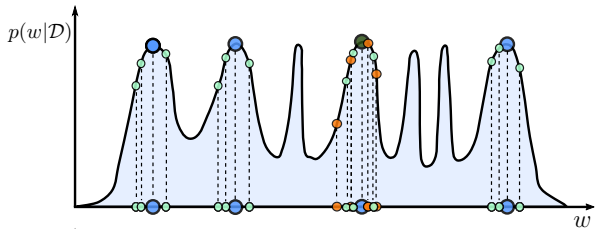
\includegraphics[width=0.7\linewidth]{./Figures/multiswag.png}
	\caption{Figure 3 from \textcite{wilson2020bayesian}: How deep ensembles (blue), VI (orange), and multi-SWAG (green) sample from the posterior.
	Deep ensembles only find different modes, VI finds one mode and explores the nearby region, and multi-SWAG finds different modes and explores the nearby regions.}
	\label{fig:multiswag}
\end{figure} 

%\subsubsection{Discussion}

\subsection{Model comparison}

Model comparison refers to selecting between different priors and hyperpriors, between different hyperparameter values and between different models $\cH$. 

\subsubsection{Hyperparameters: optimize, sample or integrate out upfront?}

As shown in Section~\ref{sec:hyperpriors}, the posterior $p(\bw|\cD,\cH)$ is obtained by integrating out the hyperparameters based on their posterior $p(\alpha,\beta|\cD,\cH)$ given by Eq.~\eqref{posterior_hypers}. 
According to this procedure, there are two levels of inference, i.e., inference of the hyperparameters via Eq.~\eqref{posterior_hypers} and inference of the parameters via Eq.~\eqref{posterior_params} given the inferred hyperparameters. 
However, the integral of Eq.~\eqref{posterior_2} is typically intractable.

One workaround is to approximate Eq.~\eqref{posterior_2} as
\begin{equation}\label{posterior_3}
p(\bw|\cD,\cH) \approx p(\bw|\cD,\hat{\alpha},\hat{\beta},\cH) 
\end{equation}
where $\hat{\alpha}$ and $\hat{\beta}$ are selected values satisfying some optimality condition.
An alternative, is to incorporate the hyperparameters in the posterior sampling scheme as delineated in Section~\ref{sec:mc}.
Finally, considering (only in this section) that $\beta$ is known, one could also directly infer the parameters from Eq.~\eqref{posterior} by using the so-called ``true prior'' $p(\bw|\cH)$, which is given by integrating out the hyperparameter $\alpha$ based on its hyperprior, i.e., 
\begin{equation}\label{}
p(\bw|\cH) = \int p(\bw|\alpha,\cH) p(\alpha|\cH) d\alpha
\end{equation}
Note that the above calculation is made before any data has arrived. 

A comparison of the optimization and integration alternatives in the context of Laplace approximation can be found in \textcite{mackay1994hyperparameters}. 
In summary, \textcite{mackay1994hyperparameters} proposes to optimize the hyperparameters and to follow Eq.~\eqref{posterior_3}, because although integration leads to the correct maximum of the posterior $p(\bw|\cD,\cH)$, it does not capture its probability mass. 
However, this comparison is based on the Laplace approximation.
More literature review is needed for a thorough comparison of these alternatives. 
In these notes the optimization and the sampling approaches are discussed; see also Section~\ref{sec:alternation}.

\subsubsection{Evidence framework (empirical Bayes)}\label{sec:evidence}

Suppose that in Eq.~\eqref{posterior_hypers} $p(\alpha, \beta|\cH)$ is a hyperprior that assigns equal probability to all values of $\alpha, \beta$; i.e., a non-informative prior. 
Then the hyperparameter posterior $p(\alpha, \beta|\cD,\cH)$ is given up to a constant by $p(\cD|\alpha, \beta,\cH)$, which is the evidence; note that $p(\cD|\alpha, \beta,\cH)$ is also the denominator in Eq.~\eqref{posterior_2}. 
Therefore, a way of selecting $\alpha, \beta$ is by maximizing the evidence, i.e.,  
\begin{equation}\label{evidence_max}
\hat{\alpha}, \hat{\beta} = \underset{\alpha, \beta}{\mathrm{argmax}}~p(\cD|\alpha, \beta,\cH)
\end{equation}
where 
\begin{equation}\label{evidence}
p(\cD|\alpha, \beta,\cH) = \int p(\cD|\bw,\beta,\cH)p(\bw|\alpha,\cH) d\bw
\end{equation}
This evidence maximization technique is widely used in Bayesian statistics and is also known as empirical Bayes or type II maximum likelihood estimation. 
See also \textcite{mackay1995probable} p. 35 where the evidence framework is compared with the minimum description length concept used in \textcite{hinton1993keeping} in conjunction with variational inference.
In short, \textcite{mackay1995probable} claims that with care one can replicate Bayesian results in terms of minimum description lengths and sees no advantage of using the latter. 

In this section some basic notions are introduced mainly based on the works of MacKay. 
The evidence may be hard to compute and thus hard to optimize the hyperparameters using it.
In this regard, see \textcite{neal1993probabilistic} (Section~6) and \textcite{robert2009computational} for surveys  on computational methods, as well as \textcite{sohl-dickstein2012hamiltonian}. 
Nevertheless, analytical expressions exist if the Laplace approximation is used for the posterior. 
Moreover, the evidence framework coupled with Laplace approximation gives us deep insights on effective dimensionality and generalization as noted in \textcite{maddox2020rethinking} and in Section~\ref{sec:rethinking}.
Finally, see \textcite{krishnan2019specifying} for a more modern approach to Empirical Bayes.

\paragraph{Evidence in conjunction with Laplace approximation:} 
According to Laplace approximation (Section~\ref{sec:laplace}) the parameter posterior can be obtained by Eq.~\eqref{laplace_posterior}. 
By substituting Eq.~\eqref{laplace_posterior} into Eq.~\eqref{evidence} an analytical expression (Eq.~(4.6) in \cite{mackay1992bayesian}) is obtained, which can be optimized numerically for obtaining $\hat{\alpha}, \hat{\beta}$ (see \cite{mackay1992bayesian} and \cite{mackay1992practical}). 
Specifically, optimization of the hyperparameters involves alternating the optimization of $\bw$ (around which the Gaussian is fitted) for fixed hyperparameters with re-estimation of the hyperparameters by re-evaluating the Hessian matrix for the new value of $\bw$ (see also Section~\ref{sec:alternation}).
Error bars for the hyperparameters can be obtained by approximating the evidence maximum with a Gaussian distribution. 
See also \textcite{mackay1995probable}, Sections 4.1 and 3.2, for modifications of the evidence framework for accounting for multimodal posteriors such as the ones arising in NNs and for multiple regularization constants, respectively.

\paragraph{Occam's razor:}
This is a principle of \textit{parsimony of explanations}; between two similarly performing explanations, we should prefer the simpler one. 
In this regard, the evidence framework automatically incorporates this principle. 
This is illustrated in Fig.~\ref{fig:occam_1}.
An overcomplex model can model many different datasets, but it is unlikely that the specific dataset $\cD$ was produced by that complex model (it has low evidence). 
Also a model that is too simple can model only a few out of all the possible datasets.
Thus, the specific dataset $\cD$ may have low evidence under such a model as well. 
As a result, the evidence framework incorporates automatically a trade-off between fitting the data and utilizing overcomplex models. 
\begin{figure}
	\centering
	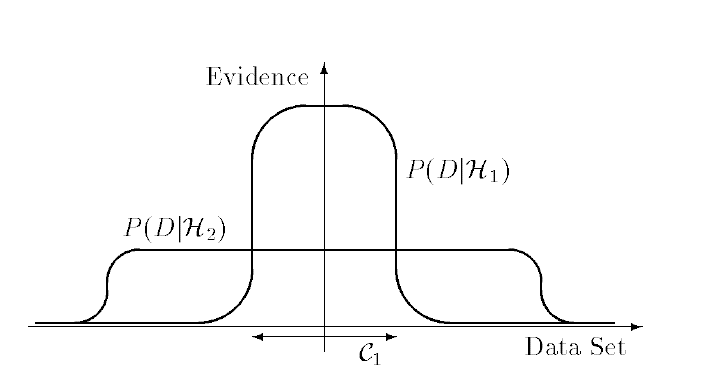
\includegraphics[width=0.7\linewidth]{./Figures/occam_1.png}
	\caption{Figure 2 from \textcite{mackay1992bayesian}: Bayes favors more probable models.
	If the dataset falls in the region $C_1$ then the less powerful model $\cH_1$ will be selected; $\cH_1$ can capture a smaller number of datasets, but because the distribution must be normalized the evidence for those datasets will be larger.}
	\label{fig:occam_1}
\end{figure} 

For an intuitive explanation, consider next Fig.~\ref{fig:occam_2}, where $\bw$ is one-dimensional ($k=1$) and $\cH_i$ denotes a specific value for the hyperparameter $\alpha$, while $\beta$ is considered known. 
For this case the evidence of Eq.~\eqref{evidence} can be approximated as 
\begin{equation}\label{evidence_occam_1}
p(\cD|\alpha, \beta,\cH) \approx p(\cD|\hat{w},\beta,\cH)p(\hat{w}|\alpha,\cH) \Delta w
\end{equation}
where $\Delta w$ is the width of the mode of the posterior. 
If the prior assigns equal probability to all values of $w$ and has width $\Delta^0 w$, Eq.~\eqref{evidence_occam_1} becomes
\begin{equation}\label{evidence_occam_2}
p(\cD|\alpha, \beta,\cH) \approx p(\cD|\hat{w},\beta,\cH) \frac{\Delta w}{\Delta^0 w}
\end{equation}
where $\frac{\Delta w}{\Delta^0 w}$ is called Occam's factor.
In summary, the evidence penalizes overcomplex models (with high prior variance $\Delta^0 w$), as well as models that need to shrink extremely in order to capture the data (too low posterior variance $\Delta w$; finely tuned to fit data). 
For a $k$-dimensional parameter vector $\bw$, Eq.~\eqref{evidence_occam_1} becomes
\begin{equation}\label{evidence_occam_3}
p(\cD|\alpha, \beta,\cH) \approx p(\cD|\hat{\bw},\beta,\cH)p(\hat{\bw}|\alpha,\cH) (2\pi)det^{-1/2}\bA
\end{equation} 
where $\bA$ denotes the Hessian of the loss given as $\bA = -\nabla\nabla\log p(\hat{\bw}|\cD,\hat{\alpha},\hat{\beta},\cH) $ and $p(\hat{\bw}|\alpha,\cH) (2\pi)det^{-1/2}\bA$ is the Occam's factor.
In the multi-dimensional case, thus, the evidence framework penalizes overcomplex models, as well as posteriors having Hessian with large determinant value.

As mentioned in \textcite{maddox2020rethinking}, more certainty about the parameters (say because of arrival of more data) leads to an increase in the curvature of the loss at the optimum.
This increase in curvature of the loss leads to an increase in the eigenvalues of the Hessian of the loss. 
Specifically, there is a gap in the eigenspectrum of the Hessian: a small number of eigenvalues become large while the rest take on values near $0$. 
Further, the directions with large eigenvalues are the ones that define effective dimensionality (see Section~\ref{sec:effective}).
Equivalently, as the eigenvalues of the Hessian increase, the eigenvalues of the covariance matrix of the posterior distribution shrink, indicating contraction around the MAP estimate. 
Once again, Occam's razor penalizes overcomplex models (small prior variance), as well as posterior contraction. 
See \textcite{maddox2020rethinking} for efficient computation of the Hessian eigenvalues and \textcite{ghorbani2019investigation} for a study on the Hessian eigenvalues in modern NNs.

Of course, the above illustrations pertain mainly to the Laplace approximation, but serve well for intuitively understanding the role of evidence. 
Most importantly, \textcite{maddox2020rethinking} relates effective dimensionality and how shrunk the posterior is with the generalization properties of NNs (see Section~\ref{sec:rethinking}).

Overall, penalizing overcomplex models \textit{arises naturally} in the Bayesian framework. 
Finally, it is worth pointing out that the variance of the prior does not necessarily affect the complexity of the output samples. 
\textcite{wilson2020bayesian} shows that for RELU NNs modifying prior variances of the layers affects only the output scale, as opposed to sigmoid NNs considered in \textcite{mackay1995probable}. 
This is an interesting topic that requires more literature review.

\begin{figure}
	\centering
	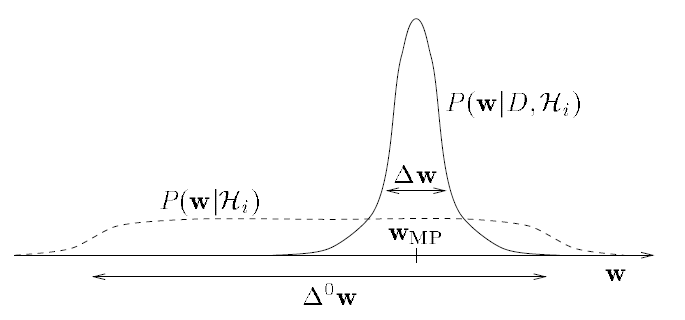
\includegraphics[width=0.7\linewidth]{./Figures/occam_2.png}
	\caption{Figure 3 from \textcite{mackay1992bayesian}: The quantities that determine Occam's factor. 
	Bayes penalizes too complex models with large $\Delta^0 w$ and shrunk posteriors with small $\Delta w$.}
	\label{fig:occam_2}
\end{figure} 

\paragraph{Effective dimensionality and generalization:}\label{sec:effective}
As mentioned above, the hyperparameters can be optimized by numerically maximizing the evidence. 
As shown in \textcite{mackay1992bayesian} however, a deeper understanding of the problem is possible by considering the properties of the maximum evidence (see also \cite{maddox2020rethinking}).
In general, given a dataset $\cD=\{y_i\}_{i=1}^N$ of $N$ Gaussian measurements with known mean $\mu$, the misfit written as
\begin{equation}
\chi^2_{\cD} = \sum_{i=1}^{N}\frac{(y_i-\mu)^2}{\sigma_{\epsilon}^2}
\end{equation}
follows a Chi-squared distribution with $N$ degrees of freedom, because we have a sum of $N$ independent random variables.
Note that in these notes $\cD$ is used for both measurements paired with their locations, i.e., $\cD=\{x_i,y_i\}_{i=1}^N$, and measurements alone, i.e., $\cD=\{y_i\}_{i=1}^N$.
In this regard, according to the discrepancy principle of statistics, we should estimate the noise level $\sigma_{\epsilon}^2$ by setting $\chi^2_{\cD} = N$, i.e., 
\begin{equation}
\hat{\sigma}_{\epsilon}^2 = \frac{\sum_i (y_i-\mu)^2}{N}
\end{equation}
However, if the mean is also estimated by the data via $\hat{\mu}=\frac{\sum_i y_i}{N}$, then we have $N-1$ independent random variables, i.e., $N-1$ degrees of freedom in the Chi-squared distribution and the noise level should be estimated by $\chi^2_{\cD}=N-1$, i.e.,
\begin{equation}
\hat{\sigma}_{\epsilon}^2 = \frac{\sum_i (y_i-\hat{\mu})^2}{N-1}
\end{equation}
In general, if $k$ free parameters are determined by the data, then we have $N-k$ degrees of freedom and $\sigma_{\epsilon}^2$ is estimated by $\chi^2_{\cD}=N-k$ (see \cite{mackay1992bayesian} for discussion).

Following the same (frequentist) rationale, the noise level $\beta = 1/\sigma_{\epsilon}^2$ in regression should be estimated by $\cL_{\cD}=N-k$, because $\bw$, which is $k$-dimensional, is estimated by the data. 
However, following the Bayesian approach of estimating the hyperparameters by maximizing the evidence, it can be shown that the resulting $\beta$ estimate satisfies, instead, the condition $\cL_{\cD}=N-\gamma$, where $\gamma = k-\alpha Trace\bA^{-1}$ represents the number of dimensions of $\bw$ that have been well-determined by the data. 
Further, the ``misfit'' from the prior, denoted as $\cL_{\bw}$, is equal to $k-(k-\gamma)=\gamma$. 
In summary, only $\gamma <k$ parameters of $\bw$ have been determined by the data, while $k-\gamma$ are determined by the prior (roughly set to zero and not contributing to reducing the training error).

Next, as stated in \textcite{mackay1992practical}, sampling theory predicts that the addition of redundant parameters to a model should reduce $\cL_{\cD}$ by one unit per well-measured parameter. 
Thus, a stopping criterion could detect the point at which as parameters are deleted, $\cL_{\cD}$ starts to increase faster than with gradient 1 with decreasing $\gamma$ (see Fig.~\ref{fig:gamma}).
This could help us \textit{select the number of hidden units}. 
\textcite{moody1991note} in a similar way penalizes large values of $\gamma$. 
In this regard, see \textcite{maddox2020rethinking} and Section~\ref{sec:rethinking} for connections between effective dimensionality, model selection and generalization behavior in modern deep learning.
\begin{figure}
	\centering
	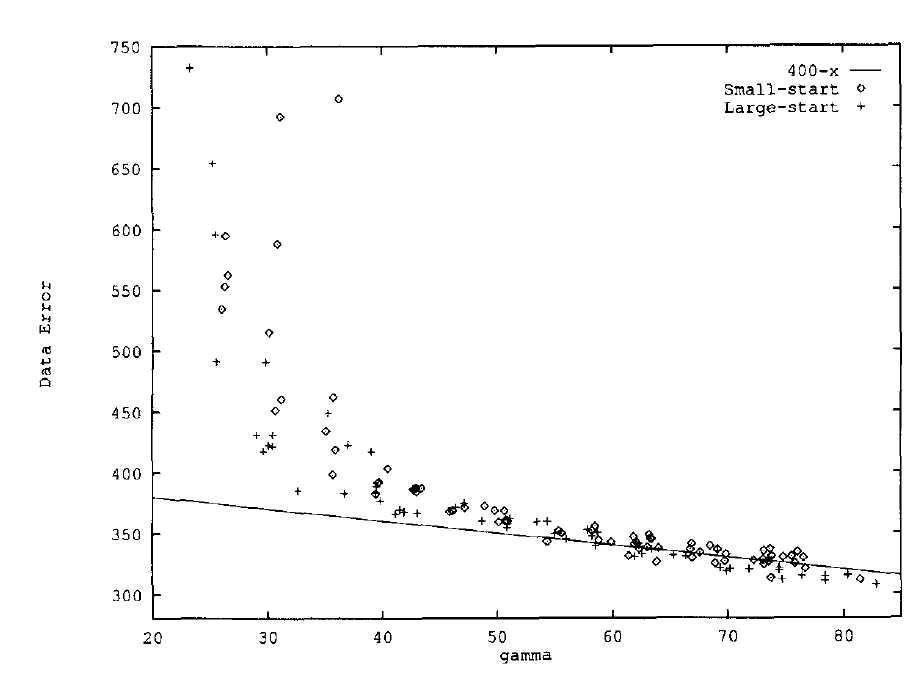
\includegraphics[width=0.7\linewidth]{./Figures/gamma.png}
	\caption{Figure 6 from \textcite{mackay1992practical}: Data misfit versus $\gamma$.
	Toward the right side of the figure, the data misfit is reduced by 1 for every well-determined parameter. 
	When the model has too few parameters, however (toward the left of the figure), the misfit gets worse at a greater rate.}
	\label{fig:gamma}
\end{figure} 

\paragraph{Rethinking parameter counting:}\label{sec:rethinking} \textcite{maddox2020rethinking} shows that effective dimensionality (having been obtained from \textit{training data only}) can be a better proxy for generalization than naive parameter counting. 
Specifically, in overparametrized cases ($k \gg N$) many dimensions of the posterior are left unchanged from the prior. 
As a result, the effective dimensionality is substantially less than the number of parameters $k$; we are unable to determine many more parameters than we have data observations.
In this regard, \textcite{maddox2020rethinking} shows that when comparing different models, the ones with smaller effective dimensionality (less well-determined parameters) lead to better generalization and thus, should be selected.
The latter is also supported by the fact that the Occam's factor in Eq.~\eqref{evidence_occam_3} does not only penalize models with too many parameters (these models have small $p(\hat{\bw}|\alpha,\cH)$), but also models with shrunk posteriors (these models have small $det^{-1/2}\bA$).

Further, a perturbation of of the MAP estimate $\hat{\bw}$ in the undetermined directions (called degenerate directions in \cite{maddox2020rethinking}) gives almost identical functions (this is called function space homogeneity).
As a result, effective dimensionality can be interpreted as model compression, since the undetermined directions do not contain additional functional information. 
Therefore, smaller effective dimensionality is interpreted as better model compression.

They show also that effective dimensionality can capture the phenomenon of double descent of the generalization performance (\cite{nakkiran2019deep}).
In short, as the model grows, there exist a greater variety of subspaces which provide more effective compression of the data, and thus we achieve a lower effective dimensionality and better generalization properties. 
This is also related to the ``blessing'' of dimensionality described in \textcite{huang2019understanding}: flat regions of the loss occupy a greatly increasing volume and thus, are more easily discoverable by optimization. 
These solutions have lower effective dimensionality and thus, provide better lossless compression of the data (\cite{maddox2020rethinking}). 

\paragraph{Should we optimize parameters and hyperparameters together in Laplace approximation?}
A point estimate of $\bw$ could be obtained by maximizing $p(\cD|\bw, \alpha,\beta,\cH) = p(\cD|\bw,\beta,\cH) p(\bw|\alpha,\cH)$ with respect to $\bw$, $\alpha$ and $\beta$ simultaneously. 
Note that $p(\cD|\bw, \alpha,\beta,\cH)$ could be regarded as the likelihood of a model that considers $\bw, \alpha$, and $\beta$ as parameters and does not distinguish between hyperparameters and parameters.
Next, this point estimate could be used either to make predictions directly using Eq.~\eqref{new_data_map} or to fit a Gaussian distribution around it (see Section~\ref{sec:laplace}). 
However, as discussed in \textcite{mackay1995developments}, this would lead to a biased estimate for the hyperparameters. 

As an example, consider the case of fitting a Gaussian (with mean $\mu$ and variance $\sigma_{\epsilon}^2$) to a dataset $\cD=\{y_i\}_{i=1}^N$. 
The maximum likelihood estimator is given as $(\hat{\mu},\hat{\sigma}_{\epsilon})=(\frac{\sum_i y_i}{N}, \frac{\sum_i (y_i-\hat{\mu})^2}{N})$, which, in frequentist terms, is biased. 
As a result, $(\hat{\mu},\hat{\sigma}_{\epsilon})=(\frac{\sum_i y_i}{N}, \frac{\sum_i (y_i-\hat{\mu})^2}{N-1})$ should be used instead.
In Bayesian terms, since we are interested in maximizing the evidence $p(\cD|\sigma_{\epsilon})$, we should average over all possible values of $\mu$ and then optimize for $\sigma_{\epsilon}$. 
Equivalently, we should optimize $p(\cD|\sigma_{\epsilon})$ and not $p(\cD|\sigma_{\epsilon}, \mu=\hat{\mu})$.
An approximation of $p(\cD|\sigma_{\epsilon})$ (or equivalently of Eq.~\eqref{evidence}) is what the evidence framework optimizes in Eq.~\eqref{evidence_max}.

Overall, in practice either an iterative approach is used that alternates between parameter inference and hyperparameter optimization, or parameter inference is performed for different values of hyperparameters and the optimal parameters are selected based on some condition (see Section~\ref{sec:alternation}). 

\paragraph{Model comparison:}  
In the same way we compare between different hyperparameter settings by comparing the resulting evidence, we can compare between different models $\cH$. 
Suppose, for example, we would like to compare between two models with different types of priors. 
This is possible by comparing $p(\cD|\cH_i)$ for different values of $i$ corresponding to different models/architectures. 
See for example Section~6 in \textcite{mackay1992bayesian}, where the error bars of the optimized hyperparameters are used for obtaining $p(\cD|\cH_i)$. 
Also see \textcite{rasmussen2001occam}, where it is claimed that automatic Occam's razor, i.e., penalization of overcomplex models, is present in both selecting hyperparameters and models. 
In both cases, evidence penalizes \textit{overcomplex functions} implied by the functional prior. 

\paragraph{Evidence in conjunction with variational inference:} 
As with Laplace approximation, optimizing the hyperparameters for the case of approximate inference by variational inference involves alternating maximization of the ELBO with respect to the posterior distribution $q$ for fixed hyperparameters and with respect to the hyperparameters for fixed $q$.

\subsubsection{Cross-validation}

In standard training of NNs cross-validation ($k$-fold typically) is predominantly used for tuning the regularization parameters.
A review of cross-validation techniques for model selection can be found in \textcite{arlot2010survey}. 
In this section its relation with evidence is briefly reviewed. 

\paragraph{Relation with evidence:} The evidence of a particular data set $\cD=\{y_i\}_{i=1}^N$ for a model $\cH$ can be written as
\begin{equation}
	p(y_1,\dots,y_N|\cH)=p(y_1|\cH)p(y_2|y_1,\cH)\cdots p(y_N|y_1,\dots,y_{N-1},\cH)
\end{equation}
where the specific permutation of data indices does not matter. 
Equivalently, the log evidence can be written as a sum of $N$ log conditionals.
Each of the $N$ terms is different depending on the particular permutation, but the sum is the same. 
The leave-one-out cross-validation error is $-\log p(y_N|y_1,\dots,y_{N-1},\cH)$ and it is a noisy error because it depends on the specific permutation. 
This is why in cross-validation the average is taken and a large data set may be required to reduce the signal to noise ratio. 
Further, \textcite{fong2020marginal} shows that the evidence is $N$ times the average leave-$p$-out cross-validation score, where the average is taken with respect to $p$.

\textcite{mackay1992bayesian} suggests that leave-one-out cross-validation is a good predictor of $-\log p(y_{N+1}|y_1,\dots,y_{N},\cH)$, i.e., of the generalization error, for large values of $N$.
However, one may not want to sacrifice useful data as a test set.
In addition, cross-validation may be computationally demanding and cannot easily handle many hyperparameters.
Finally, a large test set may be required to reduce the signal to noise ratio. 

On the other hand, the evidence may not be well-correlated with the generalization error (see Fig.~\ref{fig:evi_vs_error}); it is after all the area under the curve and may not be representative of the tail of the curve. 
If this happens we can gain useful insight into defects of the model, e.g., the regularizer may not be appropriate.
In this regard, \textcite{mackay1992practical} shows that by introducing separate hyperparameters for each layer the correlation with the generalization error is improved.
In addition, in p. 457 \textcite{mackay1992practical} suggests that $\gamma$ may serve as a useful tool for generalization error (see also \cite{maddox2020rethinking} and Section~\ref{sec:rethinking} herein).
For this reason, \textcite{mackay1992practical} proposes to do both, cross-validation and evidence computation for assessing the generalization properties of the BNN. 
\begin{figure}
	\centering
	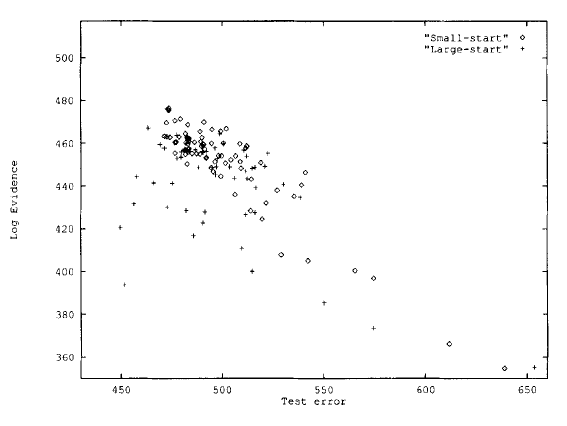
\includegraphics[width=0.7\linewidth]{./Figures/evi_vs_error.png}
	\caption{Figure 7 from \textcite{mackay1992practical}: The desired correlation between evidence and test error has negative slope.
	However, a significant number of points on the lower left side of the figure violate this desired trend.}
	\label{fig:evi_vs_error}
\end{figure} 

\subsubsection{Alternating between approximate inference and hyperparameter optimization}\label{sec:alternation}

In conclusion, either a two-step approach is followed, i.e., approximate inference and then hyperparameter optimization, or an iterative approach, i.e., alternation between approximate inference and hyperparameter optimization. 
As pointed out by \textcite{neal1998view}, there is a relation between the variational framework (variational inference combined with hyperparameter optimization) and the expectation maximization (EM) algorithm by regarding the parameter vector $\bw$ as a latent variable. 
Specifically, the E-step corresponds to ELBO maximization with respect to $q$ (Section~\ref{sec:vi}) and the M-step corresponds to optimization of the hyperparameters (see also \cite{barber1998ensemble} for discussion, \cite{gal2016uncertainty} p. 25, as well as \cite{jospin2020handson} algorithm 3). 

An alternative technique in the spirit of alternation is using Gibbs sampling steps to update the hyperparameters as done in \textcite{neal1995bayesian} and \textcite{nalisnick2018priors}.
Specifically, \textcite{neal1995bayesian} does not optimize the hyperparameters, but attempts to approximate the predictive distribution via Eq.~\eqref{new_data_hypers} by obtaining samples from $p(\bw,\alpha,\beta|\cD,\cH)$ instead of $p(\bw|\cD,\hat{\alpha},\hat{\beta},\cH)$ for optimal values $\hat{\alpha},\hat{\beta}$. 
This is done by a ``global'' Gibbs sampling scheme (Section~\ref{sec:gibbs}): The parameters $\bw$ are updated from the conditional $p(\bw|\cD,\alpha,\beta,\cH)$ via HMC (Section~\ref{sec:hmc}) for given hyperparameters $\alpha,\beta$ and then $\alpha,\beta$ are drawn from $p(\alpha,\beta|\cD,\bw,\cH)$ given the last update of the parameters $\bw$. 
See, for example, Eq. (3.17) in \textcite{neal1995bayesian} for an indicative form of the conditional $p(\alpha,\beta|\cD,\bw,\cH)$. 

\subsection{Uncertainty quality}\label{sec:quality}
As discussed in Sections~\ref{sec:classcalibration}-\ref{sec:calib}, BNNs calibrate the predictions of NNs by incorporating epistemic uncertainty.
However, \textcite{foong2019expressiveness} notes that BNNs have yet to become mainstream in deep learning, in part due to concerns raised regarding the quality of this uncertainty.
Precisely, the BNN output is obtained by the approximate inference techniques described in Section~\ref{sec:inference}, which have an effect on the uncertainty quality.

We need metrics for measuring the quality of the obtained uncertainty, as well as methods for improving it. 
One aspect of uncertainty quality is \textit{calibration}.
Calibration is measured typically with scoring rules, briefly discussed in \textcite{lakshminarayanan2017simple}.
Another aspect is \textit{sharpness}; in a regression context, this means that the confidence intervals should all be as tight as possible around a single value (\cite{kuleshov2018accurate}).
Further, improving the obtained uncertainty is related to \textit{recalibration}, discussed in Sections~\ref{sec:classcalibration} and \ref{sec:recalib}.

\subsubsection{In-domain uncertainty}
In-domain uncertainty of the model is measured on data taken from the training data distribution, i.e. data from the same domain.
\textcite{kuleshov2018accurate} notes that, in practice, Bayesian uncertainty estimates often fail to capture the true data distribution; e.g., a $90 \%$ posterior credible interval generally does not contain the true outcome $90 \%$ of the time (Fig.~\ref{fig:calib}).
\begin{figure}
	\centering
	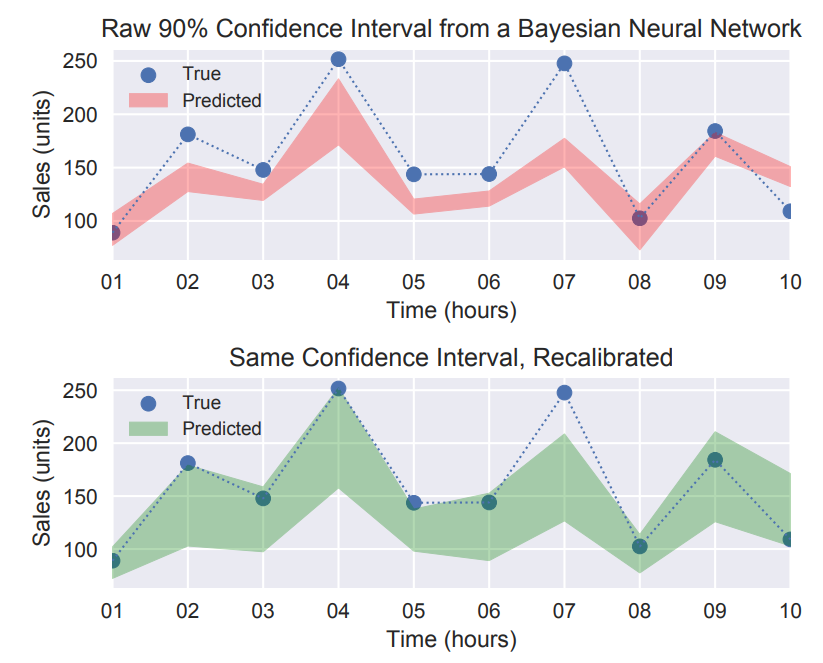
\includegraphics[width=0.7\linewidth]{./Figures/calib.png}
	\caption{Figure 1 from \textcite{kuleshov2018accurate}: 
	Top: Time series forecasting using a Bayesian neural network.
	Because the model is probabilistic, a $90\%$ credible interval around the forecast can be obtained (red). 
	However, the interval fails to capture the true data distribution: most points fall outside of it. 
	Bottom: The recalibration method proposed in \textcite{kuleshov2018accurate} enables the original model to output a $90\%$ credible interval (green) that correctly contains $9/10$ points.}
	\label{fig:calib}
\end{figure} 

\subsubsection{In-between uncertainty}
Out-of-domain or out-of-distribution uncertainty of the model is measured on the data that does not follow the same distribution as the training dataset (out-of-distribution data).
An example of out-of-distribution data is the region located in-between regions that contain training samples (Fig.~\ref{fig:inbetween}).
\textcite{foong2019inbetween} shows that mean field variational inference (VI of Section~\ref{sec:vi} with fully factorized $q_{\bth}(\bw)$; MFVI) fails to represent in-between uncertainty: its error bars are of similar magnitude in the data region and the in-between region, thus it is overconfident (Fig.~\ref{fig:inbetween}). 
The same authors provide theoretical results in \textcite{foong2019expressiveness}. 
In short, they show how the uncertainty quality depends on the expressiveness of $q_{\bth}(\bw)$.
\begin{figure}
	\centering
	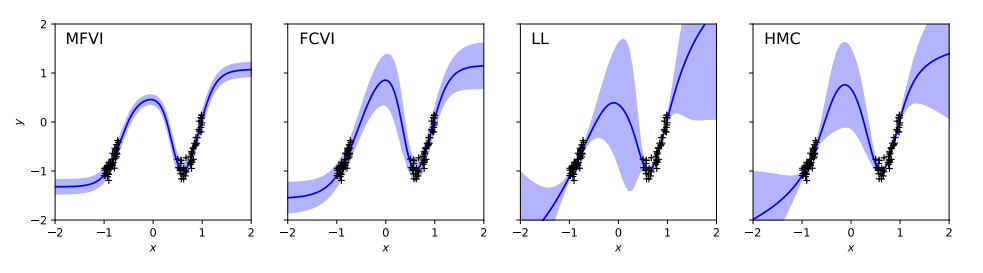
\includegraphics[width=1\linewidth]{./Figures/inbetween.png}
	\caption{Figure 1 from \textcite{foong2019inbetween}: Mean and two standard deviation bars of the predictive distribution obtained with MFVI, full covariance VI (see Section~\ref{sec:vi}), Laplace approximation and HMC.}
	\label{fig:inbetween}
\end{figure} 

\subsubsection{Recalibration of regression BNNs}\label{sec:recalib}
In general, for some input value $x_t$ the BNN outputs a cumulative distribution function (CDF) $F_{x_{t}}(y)$, or for notation simplicity, $F_{t}(y)$.
This CDF is related to $p(y^*|x^*, \cD, \cH)$ in Eq.~\eqref{new_data_2}, but the notation of \textcite{kuleshov2018accurate} is followed in this section. 
The BNN is calibrated if 
\begin{equation}
	\frac{\sum_{t=1}^{T} \textbf{1}\{y_t\leq F_t^{-1}(p)\}}{T} \to p
\end{equation}
for all $p \in [0,1]$, as $T \to \infty$. 
In other words, the empirical and the predicted CDFs should match as the dataset size goes to infinity. 
Note that the above definition does not distinguish between different locations $x_t$; the BNN is \textit{on average} calibrated. 
When the values $x_t$, $y_t$ are i.i.d. realizations of random variables $X$, $Y$ coming from the data-generating distribution, then a sufficient condition for calibration is
\begin{equation}\label{calibregres}
P(Y\leq F_X^{-1}(p)) = p
\end{equation}
Note that Eq.~\eqref{calibregres} is similar to Eq.~\eqref{classcalibr}.
Again, this is a probability over the random variable $X$ that denotes the input in general, and not a specific $x$ location.

\textcite{kuleshov2018accurate} proposes to train an auxiliary model $R:[0,1] \to [0,1]$, which takes as input the CDF $F_t$ and produces a recalibrated one, i.e., $R \circ F_t$. 
This can be done by estimating from data the probability $P(Y\leq F_X^{-1}(p))$. 
As an example, consider that for $x_t=3$ the output $F_t$ predicts $F_t(20) = 0.95$. 
This means that the $95 \%$ quantile is $F_t^{-1}(0.95) = 20$. 
If, however, our data-based estimate for $P(Y\leq F_X^{-1}(p))$ predicts that $P(Y < 20) = 0.8$, then we set $F_t(20) = 0.8$. 
We can do that for a number of quantiles, e.g., for $5 \%, 10 \%$, etc. 
The effect of recalibration is shown in Fig.~\ref{fig:calib}.
Criticism and extensions of this approach can be found in \textcite{levi2019evaluating}, \textcite{song2019distribution}, \textcite{cui2020calibrated}, and \textcite{zelikman2020crude}.

\subsubsection{Diagnostic tools}
\paragraph{Calibration:}
According to \textcite{kuleshov2018accurate}, a calibration plot for regression similar to the one for classification (Fig.~\ref{fig:reliab}) can be constructed. 
We divide the confidence axis into $M$ intervals and for each one we compute the empirical frequency
\begin{equation}
	\hat{p}_m = \frac{|\{y_t | F_t(y_t)\leq p_m, t=1,\dots,T\}|}{T}
\end{equation}
and plot $\{(p_m,\hat{p}_m)\}_{m=1}^M$. 
Calibrated forecasts correspond to a straight line.
For best results, the diagnostic dataset should be distinct from the calibration and training sets.
We can also obtain a single numerical score describing the quality of forecast calibration given by
\begin{equation}
score= \sum_{m=1}^{M}(p_m-\hat{p}_m)^2
\end{equation}

\paragraph{Sharpness:}
Sharpness can be measured using the variance of the predictions. 
Low-variance predictions are tightly centered around one value.
A sharpness score can be defined by
\begin{equation}
	sharpness = \frac{1}{T}\sum_{t = 1}^{T} var(F_t)
\end{equation}
i.e., the mean output variance of the members of the diagnostic set. 

%%%%%%%%%%%%%%%%%%%%%%%%%%%%%%%%%%%%%%%%%%%%%%%%%%%%%%%%%%%%%%%%%%%%%%%%%%%%%%%%%%%%%%%%%%%%%%%%%%%%%%%%%	

%\section*{Appendix}
\newpage	
\printbibliography[heading=bibintoc,title={References}]
	
\end{document}